\chapter{Discrete Mechanics for Rigid Bodies on Lie Groups}
\label{chapter:discrete_mechanics_for_rigid_bodies_on_lie_groups}

This chapter introduces the discrete mechanics of rigid bodies on Lie groups
for trajectory optimization computations. Thereby, it is the discrete-time 
version of the continuous mechanics in Chapter~\ref{chapter:continous_mechanics_of_rigid_bodies_on_lie_groups}. 
Instead of applying standard numerical integration methods, for example, 
the midpoint or trapezoidal rule, directly to the 
continuous equations of motion, variational integrators discretize Hamilton's 
principle. Therefore, the resulting discrete flow 
preserves the variational and geometric structure of the mechanical system 
\cite{Marsden2001,Leimkuhler_Reich_2005}. 
In correspondence with \cite{Lee2008}, the discrete time nodes 
are defined by
\begin{align*}
    t_k=t_0+kh,
    \qquad
    k=0,\ldots,N, 
    \qquad
    \text{and}
    \qquad
    Nh=t_f-t_0,
    \label{eq:discrete_time_grid}
\end{align*}
for a fixed time step $h>0$ and $N$ time steps.

Section~\ref{sec:discrete_lagrangian_mechanics} introduces the forced discrete
Euler-Lagrange equations, including the discrete Legendre transformation, and the 
geometric properties of the discrete Lagrangian flow. Additionally, a computational
approach is given for solving the implicit discrete equations. 
Subsequently, in Section \ref{sec:single_rigid_body_systems}, the formulation 
is applied to a single rigid body system and extended to 
multi-body systems in maximal coordinates in Section \ref{sec:multi_body_systems}. 
These discrete models are used for the geometric trajectory optimization
formulation and computation in 
Chapter~\ref{chapter:certifiable_trajectory_optimization}.

\section{Discrete Lagrangian Mechanics}
\label{sec:discrete_lagrangian_mechanics}

Following the continuous Lagrangian mechanics in 
Chapter \ref{chapter:continous_mechanics_of_rigid_bodies_on_lie_groups}, 
discrete Lagrangian mechanics is based on the discrete variational principle.
The continuous trajectory is replaced by 
a sequence of configurations on the Lie group, and the action integral is 
approximated by an action sum. For a regular discrete Lagrangian, the resulting Lie group 
variational integrator defines a symplectic discrete flow that remains on the configuration 
manifold. If the discrete Lagrangian is invariant under a lifted Lie-group action, the 
associated discrete 
momentum map is preserved exactly at every time step 
manifold \cite{Marsden2001,Lee2008}.

Figure~\ref{fig:discrete_mechanics} summarizes the general method for deriving the 
discrete Euler--Lagrange equations of a mechanical system on a Lie group.
Thereby, the discrete Euler-Lagrange equations are obtained from the variation
of the action sum. Alternatively, the discrete Legendre transformation can be used
to derive the discrete Hamiltonian equations of motion.

\begin{figure}[ht]
    \centering
    \resizebox{\textwidth}{!}{%
    \begin{tikzpicture}[
        node distance=0.9cm and 1.2cm,
        box/.style={
            draw, rectangle, align=center, minimum width=4.8cm,
            minimum height=1.2cm, inner sep=6pt
        },
        arrow/.style={-Latex}
    ]
        \node[box] (manifold) {Discrete configuration state\\ $(\bm{g}_k,\bm{f}_k)\in G\times G$};
        \node[box, below=of manifold] (lagrangian) {Discrete Lagrangian\\ $L_d(\bm{g}_k,\bm{f}_k)$};
        \node[box, below left=of lagrangian, xshift=1.3cm, yshift=-0.3cm] (action) {Action sum\\ $\mathcal S_d=\sum_{k=0}^{N-1}L_d(\bm{g}_k,\bm{f}_k)$};
        \node[box, below right=of lagrangian, xshift=-1.3cm, yshift=-0.3cm] (legendre) {Discrete Legendre transforms\\ $\bm{\mu}_k = \mathbb{F} L_d(\bm{g}_k,\bm{f}_k)$};
        \node[box, below=of action] (variation) {Variation\\ $\delta\mathcal S_d=0$};
        \node[box, below=of legendre] (hamilton) {Discrete Hamilton equations};
        \node[box, below=of variation] (euler) {Discrete Euler--Lagrange equations};

        \draw[arrow] (manifold) -- (lagrangian);
        \draw[arrow] (lagrangian) -- (action);
        \draw[arrow] (lagrangian) -- (legendre);
        \draw[arrow] (action) -- (variation);
        \draw[arrow] (legendre) -- (hamilton);
        \draw[arrow] (variation) -- (euler);
    \end{tikzpicture}%
    }
    \caption{General method to derive the discrete Euler--Lagrange equations of a mechanical system on a Lie group. Adapted from \cite{Lee2008}.}
    \label{fig:discrete_mechanics}
\end{figure}

\subsection{Discrete Euler--Lagrange Equations}
\label{sec:discrete_euler_lagrange_equations}

Following \cite{Lee2008,Marsden2001}, $G$ is a matrix Lie group with Lie algebra $\mathfrak g$. 
Thereby, a discrete trajectory $\bm{g}_d$ is defined by a sequence of configurations 
$\{\bm{g}_k\}_{k=0}^{N}$, where $\bm{g}_k = \bm{g}_d(t_k)$. The discrete state space is defined on $G \times G$.
By defining the relative group element $\bm{f}_k\in G$, the discrete-time kinematic equation is given by
\begin{equation}
    \bm{g}_{k+1}=\bm{g}_k\bm{f}_k.
    \label{eq:discrete_lie_group_kinematics}
\end{equation}
Consequently, the multiplicative update guarantees that $\bm{g}_{k+1}\in G$.

The discrete Lagrangian $L_d:G\times G\rightarrow\mathbb R$
approximates the action integral of the continuous Lagrangian over the interval $[t_k,t_{k+1}]$.
\cite{Marsden2001} states that, for sufficiently small $h$ and a regular continuous Lagrangian, the exact discrete Lagrangian is defined by
\begin{equation}
    L_d^{\mathrm{exact}}(\bm{g}_k,\bm{f}_k)
    =
    \int_0^h
    L\!\left(\widetilde{\bm{g}}(t),
    \widetilde{\bm{g}}(t)^{-1}\dot{\widetilde{\bm{g}}}(t)\right)
    \,\mathrm dt,
    \label{eq:exact_discrete_lagrangian}
\end{equation}
with the boundary conditions $\widetilde{\bm{g}}(0)=\bm{g}_k, \widetilde{\bm{g}}(h)=\bm{g}_k\bm{f}_k$.
Moreover, $\widetilde{\bm{g}}:[0,h]\rightarrow G$ satisfies the continuous Euler-Lagrange 
equations \eqref{eq:continuous_euler_lagrange_lie_group} \cite{Lee2008}. 
However, in this thesis, $L_d$ is calculated using the trapezoidal rule \eqref{eq:trapezodial_rule} 
to approximate \eqref{eq:exact_discrete_lagrangian}.

The discrete action sum is given by
\begin{equation}
    \mathcal S_d
    =
    \sum_{k=0}^{N-1}L_d(\bm{g}_k,\bm{f}_k).
    \label{eq:discrete_action_sum}
\end{equation}
Similarly to the continuous action integral \eqref{eq:hamilton_principle_lie_group} and the variation of the continuous Lagrangian \eqref{eq:variation_continuous_lagrangian}, 
the discrete Hamilton principle states that the action sum is stationary
\begin{equation}
    \delta\mathcal S_d
    =
    \sum_{k=0}^{N-1}\delta L_d(\bm{g}_k,\bm{f}_k)
    = \sum_{k=0}^{N-1} \left\langle D_{\bm{g}_k}L_d(\bm{g}_k,\bm{f}_k),\delta\bm{g}_k\right\rangle
    +
    \left\langle D_{\bm{f}_k}L_d(\bm{g}_k,\bm{f}_k),\delta\bm{f}_k\right\rangle
    =0,
    \label{eq:discrete_hamilton_principle}
\end{equation}
for all possible variations of $\bm{g}_d$ with fixed endpoints at $k=0$ and $k=N$ \cite{Marsden2001}.

Analogously to the continuous variation in \eqref{eq:continuous_curve_variation_lie_group}, 
the variation of the discrete configuration sequence is defined by
\begin{equation}
    \bm{g}_k^{\epsilon}
    =
    \bm{g}_k\exp(\epsilon\bm{\eta}_k)
    \label{eq:discrete_configuration_variation}
\end{equation}
with the discrete matrix-valued curve $\{\bm{\eta}_k \}^N_{k=0}$ and $\bm{\eta}_0=\bm{\eta}_N=\bm{0}$ \cite{Lee2008}.
Using the infinitesimal variation introduced 
in \eqref{eq:infinitesimal_variation_matrix_lie_group}, it follows that
\begin{equation}
    \delta\bm{g}_k=\bm{g}_k\bm{\eta}_k=T_e\mathbb{L}_{\bm{g}_k}(\bm{\eta}_k).
    \label{eq:discrete_infinitesimal_configuration_variation}
\end{equation}
Moreover, \cite{Lee2008} derives the infinitesimal variation of $\bm{f}_k$ as
\begin{align}
    \delta\bm{f}_k
    =
    T_e\mathbb{L}_{\bm{f}_k} \cdot \left(
        -\operatorname{Ad}_{\bm{f}_k^{-1}}\bm{\eta}_k+\bm{\eta}_{k+1}
    \right)
    =\bm{f}_k\bm{X}_k,
    \label{eq:discrete_relative_group_variation}
\end{align}
with $\bm{X}_k = -\operatorname{Ad}_{\bm{f}_k^{-1}}\bm{\eta}_k+\bm{\eta}_{k+1} \in\mathfrak g$.
After substituting \eqref{eq:discrete_infinitesimal_configuration_variation} and 
\eqref{eq:discrete_relative_group_variation} into \eqref{eq:discrete_hamilton_principle},
the variation of the action sum becomes 
\begin{align}
    \delta\mathcal S_d
    =
    \sum_{k=1}^{N-1}
    \Big\langle
        &T_e^*\mathbb{L}_{\bm{f}_{k-1}} \cdot D_{\bm{f}_{k-1}}L_d(\bm{g}_{k-1},\bm{f}_{k-1})
        +T_e^*\mathbb{L}_{\bm{g}_k} \cdot D_{\bm{g}_k}L_d(\bm{g}_k,\bm{f}_k)
        \notag\\
        &-
        \operatorname{Ad}_{\bm{f}_k^{-1}}^* \cdot
        \left(T_e^*\mathbb{L}_{\bm{f}_k} \cdot D_{\bm{f}_k}L_d(\bm{g}_k,\bm{f}_k)\right),
        \bm{\eta}_k
    \Big\rangle
    =0,
    \label{eq:variation_discrete_action_sum}
\end{align}
shifting the summation index, and using $\bm{\eta}_0=\bm{\eta}_N=\bm{0}$ \cite{Lee2008}.

Since \eqref{eq:variation_discrete_action_sum} holds for all 
sequences $\{\bm{\eta}_k\}_{k=1}^{N-1}\subset\mathfrak g$, the discrete Euler-Lagrange 
equations on $G$ are defined as
\begin{subequations}
\label{eq:discrete_euler_lagrange_lie_group}
\begin{align}
    T_e^*\mathbb{L}_{\bm{f}_{k-1}} \cdot D_{\bm{f}_{k-1}}L_d(\bm{g}_{k-1},\bm{f}_{k-1})
    &-
    \operatorname{Ad}_{\bm{f}_k^{-1}}^* \cdot
    \left(T_e^*\mathbb{L}_{\bm{f}_k} \cdot D_{\bm{f}_k}L_d(\bm{g}_k,\bm{f}_k)\right)
    \notag\\
    &+
    T_e^*\mathbb{L}_{\bm{g}_k} \cdot D_{\bm{g}_k}L_d(\bm{g}_k,\bm{f}_k)
    =0,
    \label{eq:discrete_euler_lagrange_balance}\\
    \bm{g}_{k+1}&=\bm{g}_k\bm{f}_k,
    \label{eq:discrete_euler_lagrange_reconstruction}
\end{align}
\end{subequations}
\cite{Lee2008}.
Equation~\eqref{eq:discrete_euler_lagrange_balance} is the dynamical representation of the
system in the body-fixed frame, while 
\eqref{eq:discrete_euler_lagrange_reconstruction} updates 
the configuration on the Lie group. 

In order to derive the discrete Euler-Lagrange equations in the following sections, 
the definitions of the partial derivatives $D_{\bm{g}_k}L_d(\bm{g}_k,\bm{f}_k)$ and $D_{\bm{f}_k}L_d(\bm{g}_k,\bm{f}_k)$ are required. 

\begin{proposition}[Directional derivative representation of $D_{\bm{g}_k}L_d(\bm{g}_k,\bm{f}_k)$]
\label{prop:directional_derivative_discrete_g}
Let $G$ be a Lie group with Lie algebra $\mathfrak g$, and let $L_d:G\times G\rightarrow\mathbb R$ be smooth \cite{Hall2000LieGroups}. 
For any $\delta\bm{g}_k=T_e\mathbb{L}_{\bm{g}_k}(\bm{\eta}_k)=\bm{g}_k\bm{\eta}_k \in T_{\bm{g}_k}G$ \eqref{eq:discrete_infinitesimal_configuration_variation}, the partial derivative $D_{\bm{g}_k}L_d(\bm{g}_k,\bm{f}_k)\in T_{\bm{g}_k}^*G$ is characterized by
\begin{equation}
    \left\langle D_{\bm{g}_k}L_d(\bm{g}_k,\bm{f}_k),\delta\bm{g}_k\right\rangle
    =
    \left\langle T_e^*\mathbb{L}_{\bm{g}_k} \cdot D_{\bm{g}_k}L_d(\bm{g}_k,\bm{f}_k),\bm{\eta}_k\right\rangle
    =
    \left.\frac{\mathrm d}{\mathrm d\epsilon}\right|_{\epsilon=0}
    L_d\!\left(\bm{g}_k\exp(\epsilon\bm{\eta}_k),\bm{f}_k\right).
    \label{eq:directional_derivative_discrete_g}
\end{equation}
\end{proposition}

\begin{proof}
By definition of the infinitesimal variation $\bm{g}_k^\epsilon$ \eqref{eq:discrete_infinitesimal_configuration_variation} and the definition of the infinitesimal 
variation on matrix Lie groups \eqref{eq:infinitesimal_variation_matrix_lie_group}, the corresponding directional derivative is
\begin{equation*}
    \left\langle D_{\bm{g}_k}L_d(\bm{g}_k,\bm{f}_k),\delta\bm{g}_k\right\rangle
    =
    \left.\frac{\mathrm d}{\mathrm d\epsilon}\right|_{\epsilon=0}
    L_d\!\left(\bm{g}_k\exp(\epsilon\bm{\eta}_k),\bm{f}_k\right).
\end{equation*}
using $\left\langle D_{\bm{g}_k}L_d(\bm{g}_k,\bm{f}_k),\delta\bm{g}_k\right\rangle = D_{\bm{g}_k}L_d(\bm{g}_k,\bm{f}_k)(\delta\bm{g}_k)$.
Additionally, the directional derivative can be expressed by the covector $T_e^*\mathbb{L}_{\bm{g}_k}$ and the definition of the differential 
of the left translation $\bm{g}_k \bm{\eta}_k = T_e\mathbb{L}_{\bm{g}_k}(\bm{\eta}_k)$ defined in \eqref{eq:preliminaries_differential_left_translation}, which leads to
\begin{align*}
    \left\langle D_{\bm{g}_k}L_d(\bm{g}_k,\bm{f}_k),\delta\bm{g}_k\right\rangle
    &=
    \left\langle D_{\bm{g}_k}L_d(\bm{g}_k,\bm{f}_k),\bm{g}_k \bm{\eta}_k\right\rangle \\
    &=
    \left\langle D_{\bm{g}_k}L_d(\bm{g}_k,\bm{f}_k),T_e\mathbb{L}_{\bm{g}_k}(\bm{\eta}_k)\right\rangle \\
    &=
    \left\langle T_e^*\mathbb{L}_{\bm{g}_k} \cdot D_{\bm{g}_k}L_d(\bm{g}_k,\bm{f}_k),\bm{\eta}_k\right\rangle.
\end{align*}
\end{proof}

\begin{proposition}[Directional derivative representation of $D_{\bm{f}_k}L_d(\bm{g}_k,\bm{f}_k)$]
\label{prop:directional_derivative_discrete_f}
Let $G$ be a matrix Lie group with Lie algebra $\mathfrak g$, 
and let $L_d:G\times G\rightarrow\mathbb R$ be smooth \cite{Hall2000LieGroups}. 
For any $\delta\bm{f}_k=T_e\mathbb{L}_{\bm{f}_k}(\bm{X}_k)=\bm{f}_k\bm{X}_k\in T_{\bm{f}_k}G$ \eqref{eq:discrete_relative_group_variation}, 
the partial derivative $D_{\bm{f}_k}L_d(\bm{g}_k,\bm{f}_k)\in T_{\bm{f}_k}^*G$ is characterized by
\begin{align}
    \left\langle D_{\bm{f}_k}L_d(\bm{g}_k,\bm{f}_k),\delta\bm{f}_k\right\rangle
    &=
    \left\langle T_e^*\mathbb{L}_{\bm{f}_k} \cdot D_{\bm{f}_k}L_d(\bm{g}_k,\bm{f}_k),\bm{X}_k\right\rangle
    \notag\\
    &=
    \left.\frac{\mathrm d}{\mathrm d\epsilon}\right|_{\epsilon=0}
    L_d\!\left(\bm{g}_k,\bm{f}_k\exp(\epsilon \bm{X}_k)\right).
    \label{eq:directional_derivative_discrete_f}
\end{align}
\end{proposition}

\begin{proof}
By definition of the infinitesimal variation $\bm{f}_k^\epsilon$ \eqref{eq:discrete_relative_group_variation} and the definition of the infinitesimal 
variation on matrix Lie groups \eqref{eq:infinitesimal_variation_matrix_lie_group}, 
the corresponding directional derivative is
\begin{equation*}
    \left\langle D_{\bm{f}_k}L_d(\bm{g}_k,\bm{f}_k),\delta\bm{f}_k\right\rangle
    =
    \left.\frac{\mathrm d}{\mathrm d\epsilon}\right|_{\epsilon=0}
    L_d\!\left(\bm{g}_k,\bm{f}_k\exp(\epsilon \bm{X}_k)\right).
\end{equation*}
using $\left\langle D_{\bm{f}_k}L_d(\bm{g}_k,\bm{f}_k),\delta\bm{f}_k\right\rangle = D_{\bm{f}_k}L_d(\bm{g}_k,\bm{f}_k)(\delta\bm{f}_k)$.
Additionally, the directional derivative can be expressed by the covector $T_e^*\mathbb{L}_{\bm{f}_k}$ and the
definition of the differential of the left translation $\bm{f}_k \bm{X}_k = T_e\mathbb{L}_{\bm{f}_k}(\bm{X}_k)$ 
defined in \eqref{eq:preliminaries_differential_left_translation}, which leads to 
\begin{align*}    
\langle D_{\bm{f}_k}L_d(\bm{g}_k,\bm{f}_k),\delta\bm{f}_k\rangle
&= \langle D_{\bm{f}_k}L_d(\bm{g}_k,\bm{f}_k),\bm{f}_k \bm{X}_k \rangle \\
&= \langle D_{\bm{f}_k}L_d(\bm{g}_k,\bm{f}_k), T_e\mathbb{L}_{\bm{f}_k}(\bm{X}_k) \rangle \\
&= \langle T_e ^* \mathbb{L}_{\bm{f}_k} \cdot D_{\bm{f}_k}L_d(\bm{g}_k,\bm{f}_k), \bm{X}_k \rangle.
\end{align*}
\end{proof}

\subsection{Discrete Legendre Transformation and Hamiltonian Mechanics}
\label{sec:discrete_legendre_hamiltonian_mechanics}

Correspondingly to the continuous Legendre transformation in Section~\ref{sec:continuous_legendre_hamiltonian_mechanics}, the same discrete dynamics can be represented on the left-trivialized cotangent bundle $T^*G$ 
identified with $G\times\mathfrak g^*$. Thereby, \cite{Lee2008} defines the discrete Legendre 
transformations $\mathbb{F}^+L_d, \mathbb{F}^- L_d: G \times G \to G \times \mathfrak{g}^*$ 
as
\begin{subequations}
\label{eq:discrete_legendre_transformations}
\begin{align}
    \mathbb F^+L_d(\bm{g}_k,\bm{f}_k)
    &=
    (\bm{g}_k\bm{f}_k,\bm{\mu}_{k+1}),
    \label{eq:positive_discrete_legendre_transformation}\\
    \mathbb F^-L_d(\bm{g}_k,\bm{f}_k)
    &=
    (\bm{g}_k,\bm{\mu}_k),
    \label{eq:negative_discrete_legendre_transformation}
\end{align}
\end{subequations}
where the discrete momenta $\bm{\mu}_k,\bm{\mu}_{k+1}\in\mathfrak g^*$ are
\begin{subequations}
\label{eq:discrete_momenta}
\begin{align}
    \bm{\mu}_k
    &=
    -T_e^*\mathbb{L}_{\bm{g}_k} \cdot D_{\bm{g}_k}L_d(\bm{g}_k,\bm{f}_k)
    +
    \operatorname{Ad}_{\bm{f}_k^{-1}}^* \cdot
    \left(T_e^*\mathbb{L}_{\bm{f}_k} \cdot D_{\bm{f}_k}L_d(\bm{g}_k,\bm{f}_k)\right),
    \label{eq:negative_discrete_momentum}\\
    \bm{\mu}_{k+1}
    &=
    T_e^*\mathbb{L}_{\bm{f}_k} \cdot D_{\bm{f}_k}L_d(\bm{g}_k,\bm{f}_k).
    \label{eq:positive_discrete_momentum}
\end{align}
\end{subequations}
\cite{Marsden2001} describes that the discrete Euler-Lagrange equation \eqref{eq:discrete_euler_lagrange_balance} is equivalent to the momentum matching condition
\begin{equation}
    \mathbb F^+L_d(\bm{g}_{k-1},\bm{f}_{k-1})
    =
    \mathbb F^-L_d(\bm{g}_k,\bm{f}_k).
    \label{eq:discrete_momentum_matching}
\end{equation}
Thus, the momentum obtained from the preceding interval is equal to the momentum obtained from the following interval at the common node $\bm{g}_k$ \cite{Marsden2001}.

Using \eqref{eq:discrete_momenta}, the corresponding discrete Hamilton equations are given by
\begin{subequations}
\label{eq:discrete_hamilton_equations_lie_group}
\begin{align}
    \operatorname{Ad}_{\bm{f}_k^{-1}}^*
    \cdot
    \left(T_e^*\mathbb{L}_{\bm{f}_k} \cdot D_{\bm{f}_k}L_d(\bm{g}_k,\bm{f}_k)\right)
    &=
    \bm{\mu}_k+T_e^*\mathbb{L}_{\bm{g}_k} \cdot D_{\bm{g}_k}L_d(\bm{g}_k,\bm{f}_k),
    \label{eq:discrete_hamilton_implicit_equation}\\
    \bm{g}_{k+1}&=\bm{g}_k\bm{f}_k,
    \label{eq:discrete_hamilton_reconstruction}\\
    \bm{\mu}_{k+1}
    &=
    \operatorname{Ad}_{\bm{f}_k}^*
    \cdot
    \left(
        \bm{\mu}_k+T_e^*\mathbb{L}_{\bm{g}_k} \cdot D_{\bm{g}_k}L_d(\bm{g}_k,\bm{f}_k)
    \right).
    \label{eq:discrete_hamilton_momentum_update}
\end{align}
\end{subequations}
First, the implicit equation 
\eqref{eq:discrete_hamilton_implicit_equation} is solved for $\bm{f}_k$, 
given the state $(\bm{g}_k,\bm{\mu}_k)$. Consequently, the next 
configuration $\bm{g}_{k+1}$ and momentum $\bm{\mu}_{k+1}$ are then obtained from 
\eqref{eq:discrete_hamilton_reconstruction} and 
\eqref{eq:discrete_hamilton_momentum_update}. 
Consequently, \eqref{eq:discrete_hamilton_equations_lie_group} defines the discrete flow 
$(\bm{g}_k,\bm{\mu}_k)\mapsto(\bm{g}_{k+1},\bm{\mu}_{k+1})$ \cite{Lee2008}.

\subsection{Properties of the Discrete Lagrangian Flow}
\label{sec:properties_discrete_lagrangian_flow}

Similarly to the continuous case in Section~\ref{sec:properties_continuous_lagrangian_flow}, 
the discrete-time Lagrangian flow associated with a regular discrete Lagrangian is symplectic. 
Moreover, if the discrete Lagrangian is invariant under the lifted action of a Lie group, the 
corresponding discrete momentum map is preserved \cite{Lee2008}.
\paragraph{Symplecticity}
In contrast to the continuous case \eqref{eq:continuous_lagrangian_one_form}, 
in the discrete case, there exist two Lagrangian one-forms $\Theta_{L_d}^{+}$, $\Theta_{L_d}^{-}$ on $G \times G$ through 
boundary terms \cite{Marsden2001}, which relation is given by
\begin{align*}
    dL_d =
    \Theta_{L_d}^{+} - \Theta_{L_d}^{-}.
\end{align*}
Moreover, \cite{Marsden2001} shows that $d\Theta_{L_d}^{+}=d\Theta_{L_d}^{-}$,
as the second-order derivative $d^2L_d$ equals zero. Therefore, the discrete Lagrangian symplectic form 
is defined as $\Omega_{L_d}=d\Theta_{L_d}^{+}=d\Theta_{L_d}^{-}$, 
which is preserved by the discrete Lagrangian flow $\mathcal F_{L_d}: G \times G \to G \times G$.
Consequently,
\begin{equation}
    (\mathcal F_{L_d}^{N-1})^*\Omega_{L_d}
    =
    \Omega_{L_d},
\end{equation}
for $N-1$ discrete steps \cite{Marsden2001}.

\paragraph{Discrete Noether's theorem}
Considering the defined action of a Lie group $H$ on $G$, $\Phi: H \times G \to G$ in Section 
\ref{sec:properties_continuous_lagrangian_flow}, there exist two Lagrangian momentum maps
$J_{L_d}^+$ and $J_{L_d}^-: G \times G \to \mathfrak h^*$.

\begin{theorem}[Discrete Noether's theorem]
\label{thm:discrete_noether}
If the discrete Lagrangian $L_d : G \times G \to \mathbb{R}$ is invariant 
under the lifted action of $\Phi: H \times G \to G$, then the two discrete 
Lagrangian momentum maps are equal $J_{L_d}^+=J_{L_d}^-=J_{L_d}$, and the 
associated discrete momentum map is preserved by the discrete Lagrangian flow,
\begin{equation}
    J_{L_d}\!\left(
        \mathcal F_{L_d}^{N-1}(\bm{g}_0,\bm{f}_0)
    \right)
    =
    J_{L_d}(\bm{g}_0,\bm{f}_0),
\end{equation}
which is called discrete Noether's theorem \cite{Marsden2001}.
\end{theorem}

In contrast to the continuous Lagrangian mechanics of 
Section~\ref{sec:continuous_lagrangian_mechanics}, 
the mathematical validation of momentum preservation for discrete variational integrators of
single and multi-body systems 
is not considered in this thesis. However, their long-time energy behaviour will be 
evaluated through numerical simulations in Section \ref{sec:numerical_simulation_results}.

\subsection{Forced Discrete Euler-Lagrange Equations}
\label{sec:discrete_forced_lagrangian}

Currently, the discrete Euler-Lagrange equations \eqref{eq:discrete_euler_lagrange_lie_group} describe unforced mechanical systems. 
However, in most cases the system is subjected to external forces or control inputs. The Lagrange-d'Alembert principle can be applied to derive the forced 
Euler-Lagrange equations for continuous mechanics, given by
\begin{align}
    \delta \int_{t_0}^{t_f} L(\bm{g}, \bm{\xi})\, dt + \int_{t_0}^{t_f} \bm{u}(t) \cdot \bm{\eta}\, dt = 0,
\end{align}
with generalized forces $\bm{u}(t):[t_0, t_f] \to \mathfrak{g}^*$ acting on the system for any $\bm{\eta}=\bm{g}^{-1}\delta\bm{g}\in\mathfrak{g}$ in continuous time \cite{Lee2008}. 

In discrete time the force in the Lagrange-d'Alembert principle is approximated by 
\begin{align}
    \int_{t_k}^{t_{k+1}} \bm{u}(t) \cdot \bm{\eta}\, dt \approx \bm{u}_{d_k}^- \cdot \bm{\eta}_k + \bm{u}_{d_k}^+ \cdot \bm{\eta}_{k+1},
\end{align}
using discrete generalized forces $\bm{u}_{d_k}^{+}, \bm{u}_{d_k}^{-} \in \mathfrak{g}^*$ acting on the system at the discrete time step $k$ \cite{Lee2008}.
Therefore, corresponding to the action sum of the discrete Lagrangian \eqref{eq:discrete_action_sum}, the discrete Lagrange-d'Alembert principle is given by 
\begin{align}\label{eq:discrete_Lagrange-d_Alembert}
    \delta \sum_{k=0}^{N-1} L_d(\bm{g}_k, \bm{f}_k) + \sum_{k=0}^{N-1} \left( \bm{u}_{d_k}^- \cdot \bm{\eta}_k + \bm{u}_{d_k}^+ \cdot \bm{\eta}_{k+1} \right) = 0.
\end{align}
\cite{Lee2008} states that \eqref{eq:discrete_Lagrange-d_Alembert} is equivalent to the discrete Hamilton's principle \eqref{eq:discrete_hamilton_principle} with the additional forcing term. 
In consequence, 
the corresponding forced version 
of the unforced discrete Euler-Lagrange equations 
\eqref{eq:discrete_euler_lagrange_lie_group} is given by
\begingroup
\small
\begin{subequations}\label{eq:discrete_forced_Euler_Lagrange}
\begin{align}
    \label{eq:discrete_forced_Euler_Lagrange_Dynamics}
    &T^*_{e}\mathbb{L}_{\bm{f}_{k-1}} \cdot D_{\bm{f}_{k-1}} L_d(\bm{g}_{k-1}, \bm{f}_{k-1})
    - \operatorname{Ad}^*_{\bm{f}_{k}^{-1}} \cdot \left(T^*_{e}\mathbb{L}_{\bm{f}_{k}} \cdot D_{\bm{f}_{k}}L_d(\bm{g}_{k}, \bm{f}_{k})\right) \notag \\
    &\qquad + T^*_{e}\mathbb{L}_{\bm{g}_{k}} \cdot D_{\bm{g}_{k}} L_d(\bm{g}_{k}, \bm{f}_{k})
    + \bm{u}^-_{d_k} + \bm{u}^+_{d_{k-1}} = \bm{0},
\end{align}
\vspace{-1.2\baselineskip}
\begin{equation}\label{eq:discrete_forced_Euler_Lagrange_Kinetics}
    \bm{g}_{k+1} = \bm{g}_{k}\bm{f}_{k}.
\end{equation}
\end{subequations}
\endgroup
According to \cite{Lee2008}, for the discrete Lagrangian of the form
\begin{align}\label{eq:discrete_lagrangian_forced_special}
    L_d(\bm{g}_k, \bm{f}_k) = T_d(\bm{f}_k) - (1-c)hV(\bm{g}_k) - chV(\bm{g}_k\bm{f}_k),
\end{align}
with $T_d(\bm{f}_k)$ being the discrete kinetic energy, $V(\bm{g}_k)$ the potential energy and $c \in [0,1]$ a constant parameter, 
the discrete forces can be generalized as
\begin{align}\label{eq:discrete_forces_special}
    \bm{u}_{d_k}^{-} = (1-c)h\bm{u}_k,
    \qquad
    \bm{u}_{d_{k}}^{+} = ch\bm{u}_{k+1},
\end{align}
at the discrete time nodes $t_k$ and $t_{k-1}$. 

\subsection{Computational Implementation}

\label{sec:discrete_computational_approach}

In contrast to the continuous mechanics of Chapter \ref{chapter:continous_mechanics_of_rigid_bodies_on_lie_groups}, numerical simulations 
can be performed for discrete-time mechanical model representations. 
Therefore, a simulation framework has to be defined. To determine the 
relative attitude update $\bm{F}_k \in SO(3)$, the implicit 
Euler-Lagrange \eqref{eq:discrete_euler_lagrange_lie_group} and Hamilton equations \eqref{eq:discrete_hamilton_equations_lie_group} 
have to be solved at every time step $k$. Therefore, an efficient 
computational algorithm is required for practical numerical 
simulations, especially for complex multibody-mechanical models. 
\cite{Lee2008} proposes an approach of expressing the group element 
$\bm{F}_k \in G$ on the linear vector space of the Lie algebra, by 
using the exponential map. Thereby, the implicit equation is 
solved numerically by a Newton iteration \cite{Marsden2001} 
in $\mathbb{R}^3$.

Firstly, the implicit discrete-time Euler-Lagrange equations 
or the discrete-time Hamilton equations have to be converted into 
an equivalent vector equation in $\mathbb{R}^3$, for example, 
using the Rodrigues formula
\begin{align}\label{eq:Rodrigues}
\bm{F}
=
\exp(\hat{\bm{f}})
=
\bm{I}_{3 \times 3}
+
\frac{\sin \lVert \bm{f} \rVert}{\lVert \bm{f} \rVert}\,\hat{\bm{f}}
+
\frac{1-\cos \lVert \bm{f} \rVert}{\lVert \bm{f} \rVert^2}\,\hat{\bm{f}}^{\,2},
\end{align}
for $\bm{f} \in \mathbb{R}^3$ \cite{MarsdenRatiu1999}. However, it requires the evaluation of expensive $\sin$ and $\cos$ terms, which increase the computational time and costs. In order to improve the computational efficiency, the exponential map \eqref{eq:Rodrigues} is replaced by the Cayley transformation \cite{Arieh_Cayley_Motivation}.


\paragraph{Cayley Transformation}

The Cayley transformation is a local diffeomorphism between $\mathbb{R}^3$ and $SO(3)$, which is defined as 
\begin{align} \label{eq:Cayley}
    \bm{F}= \operatorname{Cay}(\bm{f}) = (\bm{I} + \hat{\bm{f}})(\bm{I}-\hat{\bm{f}})^{-1} = \frac{1}{1+\bm{f}^\top \bm{f}}\left((1-\bm{f}^\top \bm{f}) \bm{I}+2\hat{\bm{f}}+2\bm{f}\bm{f}^\top\right),
\end{align}
representing a rotation $\theta$ given by $\lVert \bm{f} \rVert = \tan\left(\frac{\theta}{2}\right)$ \cite{Barbero-Linan2023_Cayley_Formula}. Therefore, the Cayley transformation is subject to the constraint $\theta < \pi$, which requires the step size $h$ to be chosen sufficiently small. After substituting the Cayley transformation \eqref{eq:Cayley} 
into the implicit equations \eqref{eq:discrete_euler_lagrange_balance} or \eqref{eq:discrete_hamilton_implicit_equation}, a 
equivalent vector equation is obtained
\begin{align}\label{eq:implicit_vector_equation}
     \bm{0} = \bm{A}(\bm{f}),
\end{align}
 where $\bm{A}:\mathbb{R}^3 \to \mathbb{R}^3$ \cite{ColomboJimenez2012SO3_Cayley}.

\paragraph{Newton Iteration}

For solving the implicit vector equation \eqref{eq:implicit_vector_equation}, Newton's method is used \cite{Marsden2001}. The iteration rule is given by 
\begin{align}
\bm{f}^{(i+1)} &= \bm{f}^{(i)} - \nabla \bm{A}\!\left(\bm{f}^{(i)}\right)^{-1} \bm{A}\!\left(\bm{f}^{(i)}\right),
\end{align}
where convergence to the solution is reached until $\left\lVert \bm{f}^{(i+1)} - \bm{f}^{(i)} \right\rVert < \varepsilon_{\mathrm N}$ for a defined $\varepsilon_{\mathrm N}$. An initial guess $\bm{f}^0$ can be obtained by linearizing the vector equation \eqref{eq:implicit_vector_equation} \cite{Lee2008}. Finally, the rotation matrix $\bm{F}_k \in SO(3)$ at $k$ is calculated using the Cayley transformation \eqref{eq:Cayley}. 

\section{Single Rigid Body Systems}
\label{sec:single_rigid_body_systems}

\subsection{3D-Pendulum}
\label{sec:discrete_3D_pendulum}

In the following Section, the unforced mechanics of a three-degree-of-freedom pendulum given by \cite{Lee2008} are presented, using discrete Lagrangian mechanics of section \ref{sec:discrete_lagrangian_mechanics}. This corresponds to the equivalent discrete case of the continuous unforced 3D-pendulum of Section \ref{section:continuous_3D_pendulum}.

\paragraph{Configuration Manifold}

The discrete configuration manifold of the unforced 3D-pendulum uses the same space and body-fixed frame definitions as the continuous model. The gravity direction in the space frame is represented by the unit vector $\bm{e}_3$, and the vector from the pivot to the center of mass is $\bm{\rho}_c$ in the body frame. As in the continuous formulation of Section \ref{section:continuous_3D_pendulum}, the discrete configuration manifold is $SO(3)$. Therefore, the attitude of the 3D-pendulum is described by a rotation matrix $\bm{R}_k \in SO(3)$, which maps the body-fixed frame to the reference frame at the discrete time step $k$. \cite{Lee2008} defines the discrete-time attitude kinematics equation as
\begin{equation}\label{eq:discrete_attitude_kinematics_equation_SO3}
    \bm{R}_{k+1}= \bm{R}_k \bm{F}_k,
\end{equation}
with the rotation matrix $\bm{F}_k$, representing the relative attitude update between two integration steps. Additionally, \cite{Lee2008} introduces adjoint operator relations for $\bm{F} \in SO(3)$ and the skew-symmetric matrix $\hat{\bm{\eta}} \in \mathfrak{so}(3)$, which are given as
\begin{align}
\operatorname{Ad}_{\bm{F}} \hat{\bm{\eta}}
&=
\bm{F}\,\hat{\bm{\eta}}\,\bm{F}^{\top}
=
(\bm{F}\bm{\eta})^\wedge,
\\
\operatorname{Ad}^{*}_{\bm{F}} \hat{\bm{\eta}}
&=
\bm{F}^{\top}\,\hat{\bm{\eta}}\,\bm{F}
=
(\bm{F}^{\top}\bm{\eta})^\wedge.\label{eq:discrete_coadjoint}
\end{align}

\paragraph{Discrete Lagrangian}

As defined in \eqref{eq:exact_discrete_lagrangian}, the discrete Lagrangian $L_d(\bm{R}_k, \bm{F}_k):SO(3) \times SO(3) \to \mathbb{R} $ is an approximation of the action integral of the continuous Lagrangian over one time step $h$. In order to discretize the given continuous Lagrangian of \eqref{eq:continuous_3D_pendulum_lagrangian}
\begin{equation}\label{eq:discrete_3D_pendulum_lagrangian}
    L(\bm{R}, \hat{\bm{\omega}}) = T(\bm{R}, \hat{\bm{\omega}}) - V(\bm{R})
    = \frac{1}{2}\operatorname{tr}[\hat{\bm{\omega}} \bm{J}_d \hat{\bm{\omega}}^\top] + mg\, \bm{e}_3^\top \bm{R}\bm{\rho}_c,
\end{equation}
the time dependent angular velocity $\hat{\bm{\omega}}(t)$ and rotation matrix $\bm{R}(t)$ have to be represented on the discrete time interval $[t_k,t_{k+1}]$ \cite{Marsden2001}. Given the definition of the exponential \eqref{eq:matrix_exponential} for an $n\times n$ matrix $\bm{X}$,
its first-order expansion can be written as
\begin{equation}\label{eq:first_order_expansion_exponential}
    \exp(\bm{X}) = \bm{I} + \bm{X} + O(\bm{X}^2).
\end{equation}
Therefore, for small $h$, the exponential map $\bm{F}_k = \exp(h \hat{\bm{\omega}}_k)$ can be approximated using \eqref{eq:first_order_expansion_exponential}, by
\[
    \bm{F}_k = \exp(h \hat{\bm{\omega}}_k) \approx \bm{I} + h \hat{\bm{\omega}}_k.
\]
This gives the general discrete approximation of the angular velocity
\begin{equation}\label{eq:discrete_velocity_approximation}
    \hat{\bm{\omega}}_k \approx \frac{1}{h}(\bm{F}_k - \bm{I}),
\end{equation}
\cite{Lee2008}. Secondly, quadrature rules, for example, the midpoint rule and the trapezoidal rule, can be applied to create an integrator $F_{L_{d}}: (\bm{R}_0, \bm{F}_0) \to (\bm{R}_1, \bm{F}_1)$ \cite{Marsden2001}. In order to align with \cite{Lee2008}, the trapezoidal rule is applied to approximate an integral, as given by
\begin{equation}\label{eq:trapezodial_rule}
    \int_{t_k}^{t_{k+1}} f(t)\,dt
    \approx
    \frac{h}{2}\left(f(t_k)+f(t_{k+1})\right),
\end{equation}
for $h = t_{k+1}-t_k$ \cite{butcher2016numerical}. Applying \eqref{eq:trapezodial_rule} to the Lagrangian \eqref{eq:discrete_3D_pendulum_lagrangian}, it follows
\begin{align}\label{eq:discrete_potential_3D_pendulum}
    \int_{t_k}^{t_{k+1}} V(\bm{R}) \, dt
    =
    \int_{t_k}^{t_{k+1}} -mg\,\bm{e}_3^{\top} \bm{R} \bm{\rho}_c \, dt
    &\approx
    -\frac{h}{2}\, mg\,\bm{e}_3^{\top}  \bm{R}_k \bm{\rho}_c
    -
    \frac{h}{2}\, mg\,\bm{e}_3^{\top} \bm{R}_{k+1} \bm{\rho}_c \notag \\
    &=
    -\frac{h}{2}\, mg\,\bm{e}_3^{\top} \bm{R}_k \bm{\rho}_c
    -
    \frac{h}{2}\, mg\,\bm{e}_3^{\top} \bm{R}_k \bm{F}_k \bm{\rho}_c, \notag \\
    &=\frac{h}{2}V(\bm{R}_k)+\frac{h}{2}V(\bm{R}_k \bm{F}_k),
\end{align}
using \eqref{eq:discrete_attitude_kinematics_equation_SO3}, as only the potential energy $V(\bm{R})$ of the continuous Lagrangian depends on $\bm{R}$. Substituting \eqref{eq:discrete_velocity_approximation} and \eqref{eq:discrete_potential_3D_pendulum} into \eqref{eq:discrete_3D_pendulum_lagrangian}, the discrete Lagrangian is calculated as
\begin{align}\label{eq:discrete_3d_pendulum_discrete_lagrangian_full}
    L_d(\bm{R}_k,\bm{F}_k)
    &=
    \frac{1}{2h}\operatorname{tr}\!\left[(\bm{F}_k-\bm{I})\bm{J}_d(\bm{F}_k-\bm{I})^{\top}\right]
    - \frac{h}{2}\left(V(\bm{R}_k)+V(\bm{R}_k\bm{F}_k)\right)  \notag\\
    &=
    \frac{1}{2h}\operatorname{tr}\!\left[
        \bm{F}_k\bm{J}_d\bm{F}_k^{\top}
        - \bm{J}_d\bm{F}_k^{\top}
        - \bm{F}_k\bm{J}_d
        + \bm{J}_d
    \right]
    - \frac{h}{2}\left(V(\bm{R}_k)+V(\bm{R}_k\bm{F}_k)\right) \notag \\
    &=
    \frac{1}{2h}\operatorname{tr}\!\left[
        2\bm{J}_d - 2\bm{F}_k\bm{J}_d
    \right]
    - \frac{h}{2}\left(V(\bm{R}_k)+V(\bm{R}_k\bm{F}_k)\right) \notag \\
    &=
    \frac{1}{h}\operatorname{tr}\!\left[(\bm{I}-\bm{F}_k)\bm{J}_d\right]
    - \frac{h}{2}\left(V(\bm{R}_k)+V(\bm{R}_k\bm{F}_k)\right),
\end{align}
using $\operatorname{tr}[\bm{F}_k \bm{J}_d \bm{F}_k^\top] = \operatorname{tr}[\bm{J}_d \bm{F}_k^\top \bm{F}_k ] = \operatorname{tr}[\bm{J}_d]$ and $\operatorname{tr}[\bm{J}_d \bm{F}_k^\top] = \operatorname{tr}[\bm{F}_k \bm{J}_d]$, since $\bm{J}_d$ is defined as a diagonal matrix $\bm{J}_d = \bm{J}_d^\top$ \cite{Lee2008}.

\paragraph{Discrete Euler-Lagrange Equations}

In order to define the Euler-Lagrange Equation \eqref{eq:discrete_euler_lagrange_lie_group}, the derivatives of \eqref{eq:discrete_3d_pendulum_discrete_lagrangian_full} have to be calculated. Firstly, the directional derivative $\left\langle D_{\bm{F}_k}L_d(\bm{R}_k, \bm{F}_k), \delta \bm{F}_k \right\rangle = \left\langle
T_e^*\mathbb{L}_{\bm{F}_k}\,D_{\bm{F}_k}L_d(\bm{R}_k,\bm{F}_k),
\hat{\bm{X}}_k
\right\rangle$ is given by applying Proposition \eqref{prop:directional_derivative_discrete_f}, which yields
{\small
\begin{align}
\left\langle
T_e^*\mathbb{L}_{\bm{F}_k}\,D_{\bm{F}_k}L_d(\bm{R}_k,\bm{F}_k),
\hat{\bm{X}}_k
\right\rangle
&=
\left.\frac{d}{d\epsilon}\right|_{\epsilon=0}
L_d\!\left(
\bm{R}_k,\bm{F}_k\exp(\epsilon\hat{\bm{X}}_k)
\right)
\notag\\
&=
-\frac{1}{h}\operatorname{tr}\!\left[
\bm{F}_k\hat{\bm{X}}_k \bm{J}_d
\right]
+\frac{h}{2}mg\,\bm{e}_3^{\top}\bm{R}_k\bm{F}_k
\hat{\bm{X}}_k\bm{\rho}_c
\notag\\
&=
-\frac{1}{h}\operatorname{tr}\!\left[
\hat{\bm{X}}_k\bm{J}_d\bm{F}_k
\right]
+\frac{h}{2}mg\,
\left((\bm{R}_k \bm{F}_k)^{\top}\bm{e}_3\right)^{\top}
\hat{\bm{X}}_k\bm{\rho}_c,
\notag
\end{align}}
using the trace identity $\operatorname{tr}[\bm{A}\bm{B}\bm{C}] = \operatorname{tr}[\bm{B}\bm{C}\bm{A}]$ for any $\bm{A}, \bm{B}, \bm{C} \in \mathbb{R}^{n \times n}$. Additionally, \cite{Lee2008} introduces the relation $\operatorname{tr}[\hat{\bm{s}}\bm{B}] = - \left\langle \bm{B}-\bm{B}^\top, \hat{\bm{s}} \right\rangle$ for any $\bm{s} \in \mathbb{R}^3,\bm{B} \in \mathbb{R}^{3 \times 3}$. Applying it together with $\bm{a}^\top \hat{\bm{x}}\bm{b} = (\bm{b} \times \bm{a}) \cdot \bm{x}$ for any $\bm{a}, \bm{b}, \bm{x} \in \mathbb{R}^3$, the inner product definition \eqref{eq:trace_inner_product}, and the linearity of the pairing $\left\langle \bm{A}, \bm{B} \right\rangle + \left\langle \bm{C}, \bm{B} \right\rangle = \left\langle \bm{A}+\bm{C},\bm{B} \right\rangle$ for any $\bm{A}, \bm{B}, \bm{C} \in \mathbb{R}^{n \times n}$, the final directional derivative of the discrete Lagrangian with respect to $\bm{F}_k$ is calculated as
{\small
\begin{align}
\left\langle
T_e^*\mathbb{L}_{\bm{F}_k}\,D_{\bm{F}_k}L_d(\bm{R}_k,\bm{F}_k),
\hat{\bm{X}}_k
\right\rangle
&=
\left\langle
\frac{1}{h}
\left(\bm{J}_d\bm{F}_k-\bm{F}_k^{\top}\bm{J}_d\right),
\hat{\bm{X}}_k
\right\rangle
+\left\langle
\frac{h}{2}mg\,
\left(
\bm{\rho}_c\times (\bm{R}_k\bm{F}_k)^{\top}\bm{e}_3
\right)^\wedge,
\hat{\bm{X}}_k
\right\rangle
\notag\\
&=
\left\langle
\frac{1}{h}
\left(\bm{J}_d\bm{F}_k-\bm{F}_k^{\top}\bm{J}_d\right)
+
\left(
\frac{h}{2}mg\,
\bm{\rho}_c\times \bm{R}_{k+1}^{\top}\bm{e}_3
\right)^\wedge,
\hat{\bm{X}}_k
\right\rangle. \notag
\end{align}}
Therefore,
\begin{equation}\label{eq:discrete_3D_pendulum_derivative_fk}
    T_e^*\mathbb{L}_{\bm{F}_k}\,D_{\bm{F}_k}L_d(\bm{R}_k,\bm{F}_k)
    \;\widehat{=}\;
    \frac{1}{h}\left(\bm{J}_d \bm{F}_k - \bm{F}_k^{\top}\bm{J}_d\right)
    +
    \frac{h}{2}\,\hat{\bm{\tau}}_{g,k+1},
\end{equation}
    with the definition of
\begin{equation}\label{eq:3d_pendulum_gravity_moment}
    \bm{\tau}_{g,k} = mg\,\bm{\rho}_c\times \bm{R}_{k}^{\top}\bm{e}_3,
\end{equation}
being the moment due to the potential energy in the body frame \cite{Lee2008}.

Moreover, the directional derivative 
\[
\left\langle
D_{\bm{R}_{k+1}}L_d(\bm{R}_{k+1},\bm{F}_{k+1}),
\delta \bm{R}_{k+1}
\right\rangle = \left\langle
T_e^*\mathbb{L}_{\bm{R}_{k+1}}\,D_{\bm{R}_{k+1}}L_d(\bm{R}_{k+1},\bm{F}_{k+1}),
\hat{\bm{\eta}}_{k+1}
\right\rangle,
\] which in this model depends only on the potential energy $V(\bm{R}_{k+1})+V(\bm{R}_{k+1} \bm{F}_{k+1})$, is calculated using Proposition \eqref{prop:directional_derivative_discrete_g} as
{\small
\begin{align}
\left\langle
T_e^*\mathbb{L}_{\bm{R}_{k+1}}\,D_{\bm{R}_{k+1}}L_d(\bm{R}_{k+1},\bm{F}_{k+1}),
\hat{\bm{\eta}}_{k+1}
\right\rangle
\notag
&=
\left.\frac{d}{d\epsilon}\right|_{\epsilon=0}
L_d\!\left(
\bm{R}_{k+1}\exp(\epsilon\hat{\bm{\eta}}_{k+1}),
\bm{F}_{k+1}
\right)
\notag\\
&=
\frac{h}{2}mg\,\bm{e}_3^{\top}\bm{R}_{k+1}\hat{\bm{\eta}}_{k+1}\bm{\rho}_c
+
\frac{h}{2}mg\,\bm{e}_3^{\top}\bm{R}_{k+1}\hat{\bm{\eta}}_{k+1}\bm{F}_{k+1}\bm{\rho}_c
\notag\\
&=
\frac{h}{2}mg
\left[
\left(\bm{\rho}_c\times \bm{R}_{k+1}^{\top}\bm{e}_3\right)
+
\left(\bm{F}_{k+1}\bm{\rho}_c\times \bm{R}_{k+1}^{\top}\bm{e}_3\right)
\right]\cdot \bm{\eta}_{k+1}.
\notag
\end{align}}
Applying the definition of inner products \eqref{eq:trace_inner_product}, it follows 
{\small
\begin{align}  
 \left\langle
T_e^*\mathbb{L}_{\bm{R}_{k+1}}\,D_{\bm{R}_{k+1}}L_d(\bm{R}_{k+1},\bm{F}_{k+1}),
\hat{\bm{\eta}}_{k+1}
\right\rangle
&=
\left\langle
\frac{h}{2}mg
\left[
\left(\bm{\rho}_c\times \bm{R}_{k+1}^{\top}\bm{e}_3\right)
+
\left(\bm{F}_{k+1}\bm{\rho}_c\times \bm{R}_{k+1}^{\top}\bm{e}_3\right)
\right]^\wedge,
\hat{\bm{\eta}}_{k+1}
\right\rangle.
\notag \\
&=
\left\langle
\frac{h}{2}
\left(
\hat{\bm{\tau}}_{g,k+1}
+
(\bm{F}_{k+1}\bm{\tau}_{g,k+2})^\wedge
\right),
\hat{\bm{\eta}}_{k+1}
\right\rangle,
\notag
\end{align}
}
which implies that the derivative of \eqref{eq:discrete_3D_pendulum_lagrangian} with respect to $\bm{R}_{k+1}$ is given by
\begin{equation}\label{eq:discrete_3D_pendulum_derivative_gk}
    T_e^*\mathbb{L}_{\bm{R}_{k+1}}\,D_{\bm{R}_{k+1}}L_d(\bm{R}_{k+1},\bm{F}_{k+1}) = \frac{h}{2}
\left[
\hat{\bm{\tau}}_{g,k+1}
+
(\bm{F}_{k+1}\bm{\tau}_{g,k+2})^\wedge
\right].
\end{equation}

Since the directional derivative
$T_e^*\mathbb{L}_{\bm{F}_k}\,D_{\bm{F}_k}L_d(\bm{R}_k,\bm{F}_k)$
was already derived in \eqref{eq:discrete_3D_pendulum_derivative_fk}, the coadjoint term in the discrete Euler-Lagrange equation \eqref{eq:discrete_euler_lagrange_lie_group} can be written in matrix form as 
{\small
\begin{align}
\operatorname{Ad}^{*}_{\bm{F}_{k+1}^{-1}}
\!\left(
T_e^*\mathbb{L}_{\bm{F}_{k+1}}
D_{\bm{F}_{k+1}}L_d(\bm{R}_{k+1},\bm{F}_{k+1})
\right)
&=
\bm{F}_{k+1}
\left[
\frac{1}{h}
\left(
\bm{J}_d\bm{F}_{k+1}
-
\bm{F}_{k+1}^{\top}\bm{J}_d
\right)
+
\frac{h}{2}\hat{\bm{\tau}}_{g,k+2}
\right]
\bm{F}_{k+1}^{\top}
\notag\\
&=
\frac{1}{h}
\left(
\bm{F}_{k+1}\bm{J}_d
-
\bm{J}_d\bm{F}_{k+1}^{\top}
\right)
+
\frac{h}{2}\bm{F}_{k+1}\hat{\bm{\tau}}_{g,k+2}\bm{F}_{k+1}^{\top}
\notag\\
&=
\frac{1}{h}
\left(
\bm{F}_{k+1}\bm{J}_d
-
\bm{J}_d\bm{F}_{k+1}^{\top}
\right)
+
\frac{h}{2}(\bm{F}_{k+1}\bm{\tau}_{g,k+2})^\wedge\label{eq:discrete_3D_pendulum_coadjoint},
\end{align}}
by using the identity \eqref{eq:discrete_coadjoint}.

Finally, the discrete Euler-Lagrange equations of the unforced 3D-pendulum are expressed in $\mathfrak{so}(3)$ $SO(3)$ form, substituting \eqref{eq:discrete_3D_pendulum_derivative_fk}, \eqref{eq:discrete_3D_pendulum_derivative_gk} and \eqref{eq:discrete_3D_pendulum_coadjoint} into \eqref{eq:discrete_euler_lagrange_lie_group}, which results in
\begin{subequations}\label{eq:discrete_3D_pendulum_EL}
\begin{align}
    \label{eq:discrete_3D_pednulum_EL_1}
    \frac{1}{h}\left(
        \bm{F}_{k+1}\bm{J}_d
        - \bm{J}_d\bm{F}_{k+1}^{\top}
        - \bm{J}_d\bm{F}_k
        + \bm{F}_k^{\top}\bm{J}_d
    \right)
    &=
    h\,\hat{\bm{\tau}}_{g,k+1}, \\
    \label{eq:discrete_3D_pednulum_EL_2}
    \bm{R}_{k+1} &= \bm{R}_k \bm{F}_k.
\end{align}
\end{subequations}
\cite{Lee2008} describes the procedure of obtaining the discrete-time flow map $(\bm{R}_{k},\bm{R}_{k+1}) \to (\bm{R}_{k+1},\bm{R}_{k+2})$ by solving \eqref{eq:discrete_3D_pednulum_EL_1} for $\bm{F}_{k+1}$ for given $(\bm{R}_{k},\bm{R}_{k+1})$ and $\bm{F}_k = \bm{R}_k^\top\bm{R}_{k+1}$. Secondly, $\bm{R}_{k+2}$ is derived from \eqref{eq:discrete_3D_pednulum_EL_2}.  

\paragraph{Discrete Legendre Transformation}

In order to obtain the discrete Hamilton equations for the unforced 3D-pendulum model, the discrete Legendre transformation $\mathbb{F}^+L_d, \mathbb{F}^-L_d:(SO(3)\times SO(3)) \to (SO(3) \times \mathfrak{so}(3)^*)$ with $\mathbb{F}^+L_d(\bm{R}_{k-1}, \bm{F}_{k-1}) = \mathbb{F}^-L_d(\bm{R}_k, \bm{F}_k)$ \eqref{eq:discrete_legendre_transformations} have to be applied. This results in the expression for the discrete momentum

\begin{subequations}\label{eq:discrete_3D_pendulum_momentum}
\begin{align}
    \hat{\bm{\Pi}}_k
    &=
    -\frac{h}{2}\left(
        \hat{\bm{\tau}}_{g,k}
        + \left(\bm{F}_k\bm{\tau}_{g,k+1}\right)^\wedge
    \right)
    +
    \frac{1}{h}\left(
        \bm{F}_k\bm{J}_d
        - \bm{J}_d\bm{F}_k^{\top}
    \right)
    +
    \frac{h}{2}\left(\bm{F}_k\bm{\tau}_{g,k+1}\right)^\wedge
    \notag \\
    &=
    \frac{1}{h}\left(
        \bm{F}_k\bm{J}_d
        - \bm{J}_d\bm{F}_k^{\top}
    \right)
    - \frac{h}{2}\hat{\bm{\tau}}_{g,k}, \label{eq:discrete_3D_pendulum_momentum_1} \\
    \hat{\bm{\Pi}}_{k+1}
    &=
    \frac{1}{h}\left(
        \bm{J}_d\bm{F}_k
        - \bm{F}_k^{\top}\bm{J}_d
    \right)
    + \frac{h}{2}\hat{\bm{\tau}}_{g,k+1},\label{eq:discrete_3D_pendulum_momentum_2}
\end{align}
\end{subequations}
where $ \hat{\bm{\Pi}} \in \mathfrak{so}(3)^*$. By substituting \eqref{eq:discrete_3D_pendulum_derivative_fk}, \eqref{eq:discrete_3D_pendulum_derivative_gk} and \eqref{eq:discrete_3D_pendulum_coadjoint} into \eqref{eq:discrete_hamilton_equations_lie_group}, the discrete Hamilton equations of an unforced 3D-pendulum are calculated as
\begin{subequations}\label{eq:discrete_3D_pendulum_hamilton}
\begin{align}
    \label{eq:discrete_3D_pendulum_hamilton_1}
     \frac{1}{h}\left(
        \bm{F}_k \bm{J}_d
        - \bm{J}_d \bm{F}_k^{\top}
    \right)
    &=
    \hat{\bm{\Pi}}_k
    + \frac{h}{2}\hat{\bm{\tau}}_{g,k} ,\\
    \label{eq:discrete_3D_pendulum_hamilton_2}
    \bm{R}_{k+1}
    &=
    \bm{R}_k \bm{F}_k ,\\
    \label{eq:discrete_3D_pendulum_hamilton_3}
    \hat{\bm{\Pi}}_{k+1}
    &=
    (\bm{F}_k^\top \bm{\Pi}_k)^\wedge
    + \frac{h}{2}(\bm{F}_k^\top \bm{\tau}_{g,k})^\wedge
    + \frac{h}{2}\hat{\bm{\tau}}_{g,k+1}.
\end{align}
\end{subequations}
Finally, the discrete map $(\bm{R}_k, \bm{\Pi}_k)  \to (\bm{R}_{k+1}, \bm{\Pi}_{k+1})$ is obtained by implicitly solving the equation \eqref{eq:discrete_3D_pendulum_hamilton_1} for $\bm{F}_k$ with given $(\bm{R}_k, \bm{\Pi}_k)$. In consequence, $\bm{R}_{k+1}$ is derived from \eqref{eq:discrete_3D_pendulum_hamilton_2}, and $\bm{\Pi}_{k+1}$ from \eqref{eq:discrete_3D_pendulum_hamilton_3}.

\paragraph{Controlled 3D Pendulum}

The derived Euler-Lagrange and Hamilton equations describe the free
motion of the 3D pendulum under the influence of gravity. In order to formulate a control problem,
an external control moment $\bm{u}_k$ is applied to the system. \cite{Lee2008} identifies 
\begin{align}\label{eq:external_control_moment_3D_pendulum}
    \bm{u}_k = \bm{R}_k^\top \bm{e}_3 \times \bm{u}_{p_{k}},
\end{align}
in the body-fixed frame for a control parameter $\bm{u}_{p_{k}} \in \mathbb{R}^3$. Thereby, the external control moment has no component
along the gravity direction, since the vector $\bm{R}_k^\top \bm{e}_3$ is aligned with the gravity vector. Thus, the
control input preserves the angular momentum about the gravity direction.

For the discrete Lagrangian in
\eqref{eq:discrete_3D_pendulum_lagrangian}, the potential energy is evaluated at
both endpoints of the time interval. Comparing its coefficients with the generalized
mechanical discrete Lagrangian \eqref{eq:discrete_lagrangian_forced_special} gives $c=\frac{1}{2}$,
which corresponds to the trapezoidal approximation of the potential contribution. Consequently, using the representation
of the generalized forces in
\eqref{eq:discrete_forces_special}, the discrete 
generalized forces are chosen as
\begin{align}\label{eq:generalized_forced_3D_pendulum}
    \bm{u}_{d_k}^{-}
    =
    \frac{h}{2}\bm{u}_k,
    \qquad
    \bm{u}_{d_{k}}^{+}
    =
    \frac{h}{2}\bm{u}_{k+1}.
\end{align}
Following, the controlled 3D-Pendulum Euler-Lagrange
equations are derived as
\begin{subequations}\label{eq:forced_3D_pendulum_EL}
\begin{align}
    \label{eq:forced_3D_pendulum_EL_dynamics}
    \frac{1}{h}\left(
        \bm{F}_{k+1}\bm{J}_d
        - \bm{J}_d\bm{F}_{k+1}^{\top}
        - \bm{J}_d\bm{F}_k
        + \bm{F}_k^{\top}\bm{J}_d
    \right)
    &=
    h\left(\bm{\tau}_{g,k+1} + \bm{u}_{k+1}\right)^\wedge,
    \\
    \label{eq:forced_3D_pendulum_EL_kinematics}
    \bm{R}_{k+1} &= \bm{R}_k \bm{F}_k.
\end{align}
\end{subequations}
by substituting the generalized forces \eqref{eq:generalized_forced_3D_pendulum} into 
the previously derived discrete Euler-Lagrange equations of the uncontrolled 
3D-pendulum \eqref{eq:discrete_3D_pendulum_EL}, considering 
the Lagrange-d'Alembert principle for forced discrete mechanics \eqref{eq:discrete_forced_Euler_Lagrange}.
Correspondingly, the controlled 3D-Pendulum Hamilton equations are given as 
\begin{subequations}\label{eq:forced_3D_pendulum_hamilton}
\begin{align}
    \label{eq:forced_3D_pendulum_hamilton_1}
    \hat{\bm{\Pi}}_k
    &=
    \frac{1}{h}\left(
        \bm{F}_k \bm{J}_d
        - \bm{J}_d \bm{F}_k^{\top}
    \right)
    - \frac{h}{2}\hat{\bm{\tau}}_{g,k}
    - \frac{h}{2}\hat{\bm{u}}_k, \\
    \label{eq:forced_3D_pendulum_hamilton_2}
    \bm{R}_{k+1}
    &=
    \bm{R}_k \bm{F}_k, \\
    \label{eq:forced_3D_pendulum_hamilton_3}
    \hat{\bm{\Pi}}_{k+1}
    &=
    (\bm{F}_k^\top \bm{\Pi}_k)^\wedge
    + \frac{h}{2}\left(\bm{F}_k^\top(\bm{\tau}_{g,k} + \bm{u}_k)\right)^\wedge
    + \frac{h}{2}(\bm{\tau}_{g,k+1} + \bm{u}_{k+1})^\wedge,
\end{align}
\end{subequations}
\cite{Lee2008}.
It can be observed that, for $\bm{u}_k=\bm{0}$, the forced discrete Euler-Lagrange \eqref{eq:forced_3D_pendulum_EL} and Hamilton \eqref{eq:forced_3D_pendulum_hamilton} equations 
reduce to the corresponding unforced equations \eqref{eq:discrete_3D_pendulum_EL}, \eqref{eq:discrete_3D_pendulum_hamilton} derived previously.
%It can be observed that, for $\bm{u}_k=\bm{0}$, the forced discrete Euler-Lagrange \eqref{eq:forced_3D_pendulum_EL} 
%reduces to the corresponding unforced equations \eqref{eq:discrete_3D_pendulum_EL}.


\section{Multi-body Systems}
\label{sec:multi_body_systems}

The previous sections considered the discrete mechanics of a single rigid body whose
configuration evolves directly on a Lie group. For multibody systems, the individual
rigid bodies are connected through mechanical joints. These joints impose holonomic
constraints on the configuration and therefore have to be included in the variational
principle. In this work, constrained multibody systems are represented in maximal
coordinates, following the formulation used for variational integrators in
maximal coordinates in \cite{BrudigamManchester2021VariationalIntegrators} and for constrained
Lie group variational dynamics in \cite{Sangli2025}.

In minimal coordinates, the configuration is described directly by the independent
degrees of freedom of the system. This representation is compact, but the
resulting kinematics and dynamics may contain nonlinear trigonometric expressions
and dense coupling terms. This is disadvantageous for the polynomial optimization
formulation considered later in this thesis. In contrast, maximal coordinates assign
each rigid body its own position and orientation variables. The reduction to the
physical degrees of freedom is then achieved by imposing algebraic joint constraints
with Lagrange multipliers. Therefore, the constraints are not artificial state
constraints, but hard mechanical constraints induced by the joints of the system
\cite{BrudigamManchester2021VariationalIntegrators}.

For a multi-body system with \(n_b\) rigid bodies in dimension
\(d\in\{2,3\}\), the maximal-coordinate configuration manifold is given by
\begin{equation}
    Q_{\mathrm{max}}
    =
    \prod_{i=1}^{n_b}
    \left(
    \mathbb{R}^{d} \times SO(d)
    \right).
    \label{eq:q_max_general}
\end{equation}
Each rigid body \(i\) is described by its center of mass position
\(\bm{x}_i\in\mathbb{R}^{d}\) and its orientation
\(\bm{R}_i\in SO(d)\). Consequently, the full configuration in maximal-coordinates is written as
\begin{equation}
    q =
    \left(
    \bm{x}_1,\bm{R}_1,\ldots,\bm{x}_{n_b},\bm{R}_{n_b}
    \right)
    \in Q_{\mathrm{max}}.
    \label{eq:q_max_state_general}
\end{equation}
The joint structure is encoded by holonomic constraints
\begin{equation}
    \bm{\phi}(q)=\bm{0},
    \qquad
    \bm{\phi}:Q_{\mathrm{max}}\rightarrow\mathbb{R}^{n_c},
    \label{eq:holonomic_constraints_general}
\end{equation}
where \(n_c\) denotes the number of scalar constraint equations.

\begin{figure}[t]
    \centering
    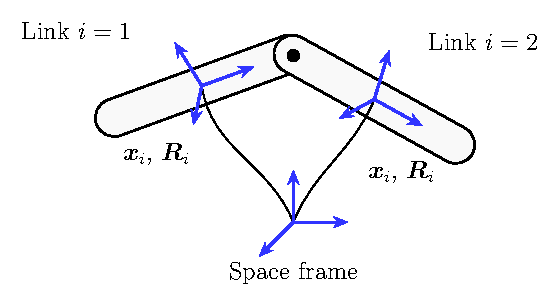
\includegraphics[width=0.65\textwidth]
        {pics/two_link_maximal_coordinates.pdf}
    \caption{Two rigid links connected by a joint in maximal coordinates.
    Adapted from \cite{BrudigamManchester2021LQR}.}
    \label{fig:maximal_coordinates_joint}
\end{figure}

A typical holonomic joint constraint can be written by equating two points
attached to different rigid bodies. This is illustrated in
Fig.~\ref{fig:maximal_coordinates_joint}. Let \(\bm{\rho}_i\) and \(\bm{\rho}_j\) denote
constant vectors from the corresponding center of mass to the joint location in
each body-fixed frame. Then a link-connecting constraint is given by
\begin{equation}
    \bm{\phi}_{ij}(q)
    =
    \bm{x}_i+\bm{R}_i\bm{\rho}_i
    -
    \bm{x}_j-\bm{R}_j\bm{\rho}_j
    =
    \bm{0}.
    \label{eq:general_joint_constraint_maximal}
\end{equation}
To include the holonomic constraints in the discrete variational principle, the
discrete action sum is augmented by Lagrange multipliers
\(\bm{\lambda}_k\in\mathbb{R}^{n_c}\). Using a trapezoidal approximation \eqref{eq:trapezodial_rule} for the
constraint contribution gives the discrete action sum
\begin{equation}
    S_{d}
    =
    \sum_{k=0}^{N-1}
    \left[
    L_d(q_k,q_{k+1})
    +
    \frac{h}{2}
    \left(
    \bm{\lambda}_k^\top \bm{\phi}(q_k)
    +
    \bm{\lambda}_{k+1}^\top \bm{\phi}(q_{k+1})
    \right)
    \right].
    \label{eq:constrained_discrete_action}
\end{equation}
%The variation with respect to \(q_k\), together with the discrete
%Lagrange--d'Alembert force contribution introduced in
%Section~\ref{sec:forced_discrete_euler_lagrange}, yields the forced and
%constrained discrete Euler-Lagrange equations
%\begin{equation}
%    D_1 L_d(q_k,q_{k+1})
%    +
%    D_2 L_d(q_{k-1},q_k)
%    +
%    \bm{u}_k
%    +
%    h\,\bm{G}(q_k)^\top \bm{\lambda}_k = 0,
%    \qquad
%    \bm{\phi}(q_k)=\bm{0},
%    \label{eq:forced_constrained_del_general}
%\end{equation}
%where
%\begin{equation}
%    \bm{G}(q_k)
%    =
%    \frac{\partial \bm{\phi}(q_k)}{\partial q_k}
%    \label{eq:constraint_jacobian_general}
%\end{equation}
%denotes the constraint Jacobian.
%Equation~\eqref{eq:forced_constrained_del_general} provides the general
%forced and constrained discrete Euler-Lagrange equation used for deriving multi-body dynamics.

\subsection{Acrobot}
\label{subsection:discrete_Acrobot}

\paragraph{Configuration Manifold}

The Acrobot model, illustrated in Fig.~\ref{fig:acrobot_maximal_coordinates},
consists of two planar rigid links connected by a revolute joint. The first link is
attached to the inertial frame by a fixed revolute joint, while the second link is
connected to the first link at the elbow. In contrast to the 3D-pendulum, the
system is described in maximal coordinates. Therefore, each link is assigned its own
center of mass position and orientation.

\begin{figure}[t]
    \centering
    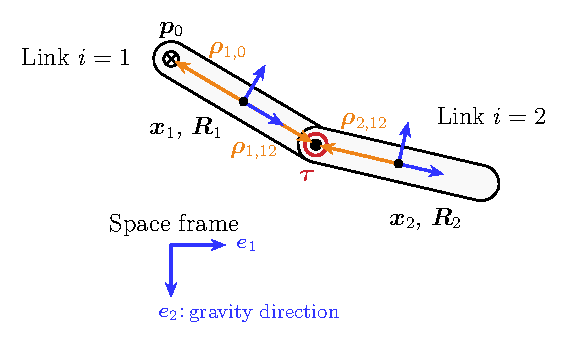
\includegraphics[width=0.75\textwidth]{pics/acrobot_maximal_coordinates.pdf}
    \caption{Acrobot configuration manifold in maximal coordinates.}
    \label{fig:acrobot_maximal_coordinates}
\end{figure}

For each link \(i\in\{1,2\}\), the center of mass position is denoted by
\(\bm{x}_i\in\mathbb{R}^2\), and the orientation of the body-fixed frame with
respect to the inertial frame is described by the rotation matrix
\(\bm{R}_i\in SO(2)\). The special orthogonal group in two dimensions is defined as
\begin{equation}
    SO(2)
    =
    \left\{
    \bm{R}\in\mathbb{R}^{2\times 2}
    \mid
    \bm{R}^{\top}\bm{R}=\bm{I}_{2},
    \ \det(\bm{R})=1
    \right\}.
    \label{eq:so2_definition}
\end{equation}
Every element \(\bm{R}_i\in SO(2)\) can be written in terms of an angle
\(\theta_i\in\mathbb{R}\) as
\begin{equation}
    \bm{R}_i
    =
    \begin{bmatrix}
        \cos\theta_i & -\sin\theta_i \\
        \sin\theta_i &  \cos\theta_i
    \end{bmatrix}.
    \label{eq:so2_rotation_matrix}
\end{equation} 
Thus, the unconstrained maximal-coordinate configuration
manifold is given by
\begin{equation}
    Q_{\mathrm{max}}
    =
    \left(
    \mathbb{R}^2 \times SO(2)
    \right)^2 .
    \label{eq:acrobot_q_max}
\end{equation}
Consequently, the constrained configuration of the Acrobot is written as
\begin{equation}
    Q_c = \{q \in Q_{\mathrm{max}} \mid \bm{\phi}(q) = \bm{0}\},
    \label{eq:acrobot_configuration}
\end{equation}
with $q = (\bm{x}_1,\bm{R}_1,\bm{x}_2,\bm{R}_2)$.
Here, \(\bm{R}_i\) maps vectors from the \(i\)-th body-fixed frame to the inertial
frame.

Let \(\bm{\rho}_{1,0}\in\mathbb{R}^2\) denote the vector from the center of mass of
link~1 to the base joint, expressed in the first body-fixed frame. Furthermore, let
\(\bm{\rho}_{1,12}\in\mathbb{R}^2\) and \(\bm{\rho}_{2,12}\in\mathbb{R}^2\) denote the
vectors from the corresponding centers of mass to the elbow joint, expressed in
the body-fixed frames of link~1 and link~2. The fixed base joint is imposed by
\begin{equation}
    \bm{\phi}_{0}(q)
    =
    \bm{x}_1
    +
    \bm{R}_1\bm{\rho}_{1,0}
    -
    \bm{p}_0
    =
    \bm{0},
    \label{eq:acrobot_base_constraint}
\end{equation}
where \(\bm{p}_0\in\mathbb{R}^2\) is the fixed base position in the inertial frame.
The elbow joint is imposed by requiring the two joint points on link~1 and link~2
to coincide, yielding
\begin{equation}
    \bm{\phi}_{12}(q)
    =
    \bm{x}_1
    +
    \bm{R}_1\bm{\rho}_{1,12}
    -
    \bm{x}_2
    -
    \bm{R}_2\bm{\rho}_{2,12}
    =
    \bm{0}.
    \label{eq:acrobot_elbow_constraint}
\end{equation}
Consequently, the full holonomic constraint vector is defined as
\begin{equation}
    \bm{\phi}(q)
    =
    \begin{bmatrix}
        \bm{\phi}_{0}(q) \\
        \bm{\phi}_{12}(q)
    \end{bmatrix}
    =
    \bm{0}.
    \label{eq:acrobot_constraints}
\end{equation}

In the discrete setting, the attitude of each link is updated by a relative rotation
\(\bm{F}_{i,k}\in SO(2)\), such that
\begin{equation}
    \bm{R}_{i,k+1}
    =
    \bm{R}_{i,k}\bm{F}_{i,k},
    \qquad i\in\{1,2\}.
    \label{eq:acrobot_rotation_update}
\end{equation}
The discrete configuration at time step \(k\) is therefore
\begin{equation}
    q_k
    =
    \left(
    \bm{x}_{1,k},\bm{R}_{1,k},
    \bm{x}_{2,k},\bm{R}_{2,k}
    \right)
    \in Q_c .
    \label{eq:acrobot_discrete_configuration}
\end{equation}

\paragraph{Continuous Lagrangian}

To derive the continuous Lagrangian of the Acrobot in maximal coordinates, the
kinetic and potential energy of both rigid links are introduced. For each link
\(i\in\{1,2\}\), the translational velocity of the center of mass is denoted by
\(\dot{\bm{x}}_i=\bm{v}_i\in\mathbb{R}^2\). Let $\bm{M}_i = m_i\bm{I}_2$ be the mass matrix of link \(i\).
The defined non-standard inertia matrix in \eqref{eq:non-standard_inertia}
is derived for $SO(3)$. In order to apply the non-standard inertia to the planar $SO(2)$ case,
the non-standard inertia matrix on \(SO(2)\) is derived by rewriting the 
planar rotational kinetic term of the discrete Lagrangian in
\cite{LeeLeokMcClamroch2007DiscreteControlSystems}. 
As a result, the relation of the non-standard
inertia to the standard inertia matrix on $SO(2)$ is given by
\begin{align}\label{eq:2D_nonstandard_inertia}
    \bm{J}_{d,i}
    =
    \frac{1}{2}J_i^{\mathrm{com}} \bm{I}_2,
\end{align}
where $J_i^{\mathrm{com}}$ is the rotational inertia of a uniform rod about its center of mass. 
The kinetic energy with its translational $T_T$ and rotational $T_R$ components is written as
\begin{equation}
    T
    =
    \underbrace{
    \sum_{i=1}^{2}
    \frac{1}{2}\bm{v}_i^{\top}\bm{M}_i\bm{v}_i
    }_{T_T}
    +
    \underbrace{
    \sum_{i=1}^{2}
    \frac{1}{2}
    \mathrm{tr}
    \left[
        \bm{\widehat{\omega}}_i
        \bm{J}_{d,i}
        \bm{\widehat{\omega}}_i^{\top}
    \right]
    }_{T_R}.
    \label{eq:acrobot_kinetic_energy_split}
\end{equation}
The gravitational potential energy is expressed directly by the center of mass
positions. In contrast to the 3D-pendulum, \cite{BrudigamManchester2021VariationalIntegrators} assumes zero potential for the rotational setting, 
which gives 
\begin{equation}
    V_R(\bm{R}_1,\bm{R}_2)=0.
    \label{eq:acrobot_rotation_potential_zero}
\end{equation}
Therefore, the gravitational potential energy is only given by the translational term
\begin{equation}
    V = V_T(\bm{x}_1,\bm{x}_2)
    =
    -
    \sum_{i=1}^{2}
    g\,\bm{e}_2^{\top}\bm{M}_i\bm{x}_i,
    \label{eq:acrobot_potential_energy}
\end{equation}
where \(\bm{e}_2\in\mathbb{R}^2\) denotes the unit vector in the gravity direction in the inertial frame.
Consequently, the continuous Lagrangian
\(L:TQ_{\mathrm{max}}\rightarrow\mathbb{R}\) is defined as
\begin{equation}
    \begin{aligned}
    L(q,\dot{q})
    &=
    \sum_{i=1}^{2}
    \left(
    \frac{1}{2}\bm{v}_i^{\top}\bm{M}_i\bm{v}_i
    +
    \frac{1}{2}
    \mathrm{tr}
    \left[
        \bm{\widehat{\omega}}_i
        \bm{J}_{d,i}
        \bm{\widehat{\omega}}_i^{\top}
    \right]
    \right)
    +
    \sum_{i=1}^{2}
    g\,\bm{e}_2^{\top}\bm{M}_i\bm{x}_i .
    \end{aligned}
    \label{eq:acrobot_continuous_lagrangian}
\end{equation}

\paragraph{Discrete Lagrangian}

In general, the discrete Lagrangian is written as
\begin{align*}
    L_d(q_k,q_{k+1})
    =
    T_{d,T}(q_k,q_{k+1})
    +
    T_{d,R}(q_k,q_{k+1})
    -
    V_{d,T}(q_k,q_{k+1}).
    \label{eq:acrobot_discrete_lagrangian_split}
\end{align*}
Following the structure of maximal-coordinate variational
integrators in \cite{BrudigamManchester2021VariationalIntegrators},
the translational and rotational parts are
discretized separately.

For the translational part, the center of mass velocity of each link is 
\begin{equation}
    \bm{v}_{i,k}
    =
    \frac{\bm{x}_{i,k+1}-\bm{x}_{i,k}}{h},
    \qquad i\in\{1,2\}.
    \label{eq:acrobot_discrete_translational_velocity}
\end{equation}
\cite{BrudigamManchester2021VariationalIntegrators} defines the discrete translational kinetic energy contribution to be
\begin{equation}
    T_{d,T}(q_k,q_{k+1})
    =
    \sum_{i=1}^{2}
    \frac{1}{2h}
    \left(
    \bm{x}_{i,k+1}-\bm{x}_{i,k}
    \right)^{\top}
    \bm{M}_i
    \left(
    \bm{x}_{i,k+1}-\bm{x}_{i,k}
    \right).
    \label{eq:acrobot_discrete_translational_lagrangian}
\end{equation}
Substituting the angular velocity approximation \eqref{eq:discrete_velocity_approximation} into the rotational kinetic energy
$T_R$ of \eqref{eq:acrobot_kinetic_energy_split}, the discrete rotational kinetic
energy contribution is derived as
\begin{equation}
\begin{aligned}
    T_{d,R}(q_k,q_{k+1})
    &=
    \sum_{i=1}^{2}
    \frac{1}{2h}
    \mathrm{tr}
    \left[
    \left(
    \bm{F}_{i,k}-\bm{I}_{2}
    \right)
    \bm{J}_{d,i}
    \left(
    \bm{F}_{i,k}-\bm{I}_{2}
    \right)^{\top}
    \right] \\
    &=
    \sum_{i=1}^{2}
    \frac{1}{h}
    \mathrm{tr}
    \left[
    \left(
    \bm{I}_{2}
    -
    \bm{F}_{i,k}
    \right)
    \bm{J}_{d,i}
    \right].
\end{aligned}
\label{eq:acrobot_discrete_rotational_lagrangian}
\end{equation}
This calculation corresponds to the discrete rotational kinetic energy of the 3D-pendulum in Section \ref{sec:discrete_3D_pendulum}.

Finally, using the trapezoidal rule for the discretization of the potential energy integral, the discrete translational potential contribution $V_{d,T}$
is given by
\begin{equation}
    V_{d,T}(q_k,q_{k+1})
    =
    -
    \frac{h}{2}
    \sum_{i=1}^{2}
    m_i g
    \bm{e}_{2}^{\top}
    \left(
    \bm{x}_{i,k}
    +
    \bm{x}_{i,k+1}
    \right).
    \label{eq:acrobot_discrete_potential_lagrangian}
\end{equation}

Combining the translational \eqref{eq:acrobot_discrete_translational_lagrangian}, rotational \eqref{eq:acrobot_discrete_rotational_lagrangian}, and potential \eqref{eq:acrobot_discrete_potential_lagrangian} contributions gives the
discrete Lagrangian
\begin{equation}
    \begin{aligned}
    L_d(q_k,q_{k+1})
    =
    &
    \text{  }
    L_d
    \left(
    \bm{x}_{1,k},\bm{x}_{1,k+1},
    \bm{x}_{2,k},\bm{x}_{2,k+1},
    \bm{F}_{1,k},\bm{F}_{2,k}
    \right)  \\
    =
    &
    \sum_{i=1}^{2}
    \frac{1}{2h}
    \left(
    \bm{x}_{i,k+1}-\bm{x}_{i,k}
    \right)^{\top}
    \bm{M}_i
    \left(
    \bm{x}_{i,k+1}-\bm{x}_{i,k}
    \right)  \\
    &
    +
    \sum_{i=1}^{2}
    \frac{1}{h}
    \mathrm{tr}
    \left[
    \left(
    \bm{I}_{2}
    -
    \bm{F}_{i,k}
    \right)
    \bm{J}_{d,i}
    \right]   \\
    &
    +
    \frac{h}{2}
    \sum_{i=1}^{2}
    g
    \bm{e}_{2}^{\top}
    \bm{M}_i
    \left(
    \bm{x}_{i,k}
    +
    \bm{x}_{i,k+1}
    \right).
    \end{aligned}
    \label{eq:acrobot_discrete_lagrangian}
\end{equation}

\paragraph{Discrete Euler-Lagrange Equations}

The discrete equations of motion are obtained from the stationary condition of the
constrained discrete action. 
The holonomic constraints introduced in
\eqref{eq:acrobot_constraints} are included by extending the action integral with
Lagrange multipliers. Let
\begin{equation}
    \bm{\lambda}
    =
    \begin{bmatrix}
        \bm{\lambda}_{0} \\
        \bm{\lambda}_{12}
    \end{bmatrix}
    \in\mathbb{R}^{4},
    \label{eq:acrobot_lagrange_multipliers}
\end{equation}
where \(\bm{\lambda}_{0}\in\mathbb{R}^2\) enforces the base constraint and
\(\bm{\lambda}_{12}\in\mathbb{R}^2\) enforces the elbow constraint.
Using the constrained action sum defined in \eqref{eq:constrained_discrete_action}, the
variation is written as
\begin{equation}
    \delta S_{d}
    =
    \delta
    \sum_{k=0}^{N-1}
    \left[
    L_d(q_k,q_{k+1})
    +
    \frac{h}{2}
    \left(
    \bm{\lambda}_{k}^{\top}\bm{\phi}(q_k)
    +
    \bm{\lambda}_{k+1}^{\top}\bm{\phi}(q_{k+1})
    \right)
    \right]
    = 0.
    \label{eq:acrobot_variation_constrained_discrete_action}
\end{equation}
The translational and rotational components are treated separately, following the
maximal-coordinate variational-integrator structure. In \cite{BrudigamManchester2021VariationalIntegrators},
the variation of the translational component is given as
\begin{equation}
    \delta_{\bm{x}_{i,k+1}} S_{d,c}
    =
    \left\langle
    \left(\frac{1}{h}\bm{M}_i
    \left(
    \bm{v}_{i,k}
    -
    \bm{v}_{i,k+1}
    \right)
    +
    g\bm{M}_i\bm{e}_2
    +
    \bm{G}_{x_i,k+1}^{\top}\bm{\lambda}_{k+1}\right) h,
    \delta\bm{x}_{i,k+1}
    \right\rangle,
    \label{eq:acrobot_translational_variation}
\end{equation}
using the relation \eqref{eq:acrobot_discrete_translational_velocity}. $\bm{G}_{x_i,k+1}$ is defined as the Jacobian of the constraints $\bm{\phi}(q_{k+1})$ with respect to $\bm{x}_{i,k+1}$.
The constraint contribution is calculated as
\begin{equation}
    \bm{G}_{x,k+1}^{\top}\bm{\lambda}_{k+1}
    =
    \begin{bmatrix}
        \dfrac{\partial \bm{\phi}_{0,k+1}}{\partial \bm{x}_{1,k+1}}
        &
        \dfrac{\partial \bm{\phi}_{0,k+1}}{\partial \bm{x}_{2,k+1}}
        \\[0.8em]
        \dfrac{\partial \bm{\phi}_{12,k+1}}{\partial \bm{x}_{1,k+1}}
        &
        \dfrac{\partial \bm{\phi}_{12,k+1}}{\partial \bm{x}_{2,k+1}}
    \end{bmatrix}^{\top}
    \begin{bmatrix}
        \bm{\lambda}_{0,k+1} \\
        \bm{\lambda}_{12,k+1}
    \end{bmatrix}  
    =
    \begin{bmatrix}
        \bm{\lambda}_{0,k+1}+\bm{\lambda}_{12,k+1} \\
        -\bm{\lambda}_{12,k+1}
    \end{bmatrix}.
    \label{eq:acrobot_translational_constraint_force}
\end{equation}
with the discretized constraints
\begin{equation}
    \bm{\phi}(q_{k+1})
    =
    \begin{bmatrix}
        \bm{\phi}_{0,k+1} \\
        \bm{\phi}_{12,k+1}
    \end{bmatrix}
    =
    \begin{bmatrix}
    \bm{x}_{1,k+1}
    +
    \bm{R}_{1,k+1}\bm{\rho}_{1,0}
    -
    \bm{p}_0
    \\
    \bm{x}_{1,k+1}
    +
    \bm{R}_{1,k+1}\bm{\rho}_{1,12}
    -
    \bm{x}_{2,k+1}
    -
    \bm{R}_{2,k+1}\bm{\rho}_{2,12}
    \end{bmatrix}.
    \label{eq:acrobot_discrete_constraints_vector}
\end{equation}
Therefore, substituting the gradient \eqref{eq:acrobot_translational_constraint_force} into \eqref{eq:acrobot_translational_variation}, the translational discrete Euler-Lagrange equations for link 1 and link 2 are
\begin{subequations}
\label{eq:acrobot_translational_del_links}
\begin{align}
    \frac{1}{h}\bm{M}_{1}
    \left(
    \bm{v}_{1,k+1}
    -
    \bm{v}_{1,k}
    \right)
    -
    g\bm{M}_{1}\bm{e}_{2}
    -
    \left(
    \bm{\lambda}_{0,k+1}
    +
    \bm{\lambda}_{12,k+1}
    \right)
    &=
    \bm{0},
    \label{eq:acrobot_translational_del_link_1}
    \\
    \frac{1}{h}\bm{M}_{2}
    \left(
    \bm{v}_{2,k+1}
    -
    \bm{v}_{2,k}
    \right)
    -
    g\bm{M}_{2}\bm{e}_{2}
    +
    \bm{\lambda}_{12,k+1}
    &=
    \bm{0}.
    \label{eq:acrobot_translational_del_link_2}
\end{align}
\end{subequations}

For the rotational part, the derivatives of \eqref{eq:discrete_euler_lagrange_lie_group} have to be taken for each link, analogously to the 3D-pendulum of Section \ref{sec:discrete_3D_pendulum}.
Firstly, the directional derivative $\left\langle D_{\bm{F}_{i,k}}L_d(\bm{F}_{i,k}), \delta \bm{F}_{i,k} \right\rangle$ is given by applying Proposition \eqref{prop:directional_derivative_discrete_f}, which yields
\begin{equation}
    \begin{aligned}
    \left\langle
    T_e^*\mathbb{L}_{\bm{F}_{i,k}}
    D_{\bm{F}_{i,k}}L_{d,R,i},
    \widehat{\bm{X}}_k
    \right\rangle
    &=
    \left.
    \frac{d}{d\epsilon}
    \right|_{\epsilon=0}
    L_{d}
    \left(
    \bm{F}_{i,k}
    \exp(\epsilon\widehat{\bm{X}}_k)
    \right)
    \\
    &=
    -
    \frac{1}{h}
    \mathrm{tr}
    \left[
    \bm{F}_{i,k}
    \widehat{\bm{X}}_k
    \bm{J}_{d,i}
    \right]
    \\
    &=
    \left\langle
    \frac{1}{h}
    \left(
    \bm{J}_{d,i}\bm{F}_{i,k}
    -
    \bm{F}_{i,k}^{\top}\bm{J}_{d,i}
    \right),
    \widehat{\bm{X}}_k
    \right\rangle
    \\
    &=
    \left\langle
    \bm{\widehat{\Pi}}_{i,k}
    ,
    \widehat{\bm{X}}_k
    \right\rangle
    , 
    \end{aligned}
    \label{eq:acrobot_rotational_derivative_pairing}
\end{equation}
corresponding to the derivative of the single body 3D-pendulum derived in Section \ref{sec:discrete_3D_pendulum}. 
Here,
\begin{equation}
    \bm{\widehat{\Pi}}_{i,k}
    =
    \frac{1}{h}
    \left(
        \bm{J}_{d,i}\bm{F}_{i,k}
        -
        \bm{F}_{i,k}^{\top}\bm{J}_{d,i}
    \right),
    \qquad i\in\{1,2\},
    \label{eq:acrobot_discrete_angular_momentum}
\end{equation}
denotes the discrete angular momentum
of link \(i\) associated with the relative rotation \(\bm{F}_{i,k}\).
It is the analogue of the discrete Legendre momentum \eqref{eq:discrete_3D_pendulum_momentum_1} used for
the 3D-pendulum in Section \ref{sec:discrete_3D_pendulum}, now defined separately for each rigid link \cite{Lee2008}.

Since \(SO(2)\) is abelian, it follows that \(\operatorname{Ad}_{\bm{F}_{i,k}}=\bm{I}\) \cite{Lee2008}.
Therefore, the coadjoint term is equal to \eqref{eq:acrobot_rotational_derivative_pairing} at time step $k+1$, which gives
\begin{equation}\label{eq:acrobot_Ad_variation}
\operatorname{Ad}^{*}_{\bm{F}_{i,k+1}^{-1}}
\!\left(
T_e^*\mathbb{L}_{\bm{F}_{i,k+1}}
D_{\bm{F}_{i,k+1}}L_d(\bm{F}_{i,k+1})
\right)
= 
\frac{1}{h}
\left(
\bm{J}_{d,i}\bm{F}_{i,k+1}
-
\bm{F}_{i,k+1}^{\top}\bm{J}_{d,i}
\right).
\end{equation}
It remains to derive the directional derivative of the rotations $\bm{R}_{i,k+1}$. 
From \eqref{eq:acrobot_variation_constrained_discrete_action}, it is observed that only the constraints $\bm{\phi}(q_k)$ are dependent on
the rotation matrices \(\bm{R}_{1,k}\) and \(\bm{R}_{2,k}\). 
Hence, the variation of the constraint contribution 
\begin{equation*}
    \left\langle D_{\bm{R}_{i,k+1}}(h \bm{\lambda}_{k+1}^\top \bm{\phi}_{k+1}), \delta \bm{R}_{i,k+1} \right\rangle=\left\langle T_e^* \mathbb{L}_{\bm{R}_{i,k+1}} D_{\bm{R}_{i,k+1}}(h \bm{\lambda}_{k+1}^\top \bm{\phi}_{k+1}), \bm{\widehat{\eta}}_{i,k+1} \right\rangle,
\end{equation*}
has to be evaluated for each link $i$, using Proposition \eqref{prop:directional_derivative_discrete_g}. For link $i=1$, the variation of the constraint contribution is given by
\begin{equation}
    \begin{aligned}
    &
    \left\langle
    T_e^*\mathbb{L}_{\bm{R}_{1,k+1}}
    D_{\bm{R}_{1,k+1}}
    \left(
    h\bm{\lambda}_{k+1}^{\top}\bm{\phi}_{k+1}
    \right),
    \bm{\widehat{\eta}}_{1,k+1}
    \right\rangle
    \\
    &=
    \left.
    \frac{d}{d\epsilon}
    \right|_{\epsilon=0}
    h
    \left[
    \bm{\lambda}_{0,k+1}^{\top}
    \bm{\phi}_{0,k+1}^{\epsilon}
    +
    \bm{\lambda}_{12,k+1}^{\top}
    \bm{\phi}_{12,k+1}^{\epsilon}
    \right]
    \\
    &=
    h 
    \left[
    \bm{\lambda}_{0,k+1}^{\top}
    \bm{R}_{1,k+1}\bm{\widehat{\eta}}_{1,k+1}\bm{\rho}_{1,0}
    +
    \bm{\lambda}_{12,k+1}^{\top}
    \bm{R}_{1,k+1}\bm{\widehat{\eta}}_{1,k+1}\bm{\rho}_{1,12}
    \right]
    \\
    &=
    h
    \left[
    \left(
    \bm{\rho}_{1,0}
    \times
    \bm{R}_{1,k+1}^{\top}\bm{\lambda}_{0,k+1}
    \right)
    +
    \left(
    \bm{\rho}_{1,12}
    \times
    \bm{R}_{1,k+1}^{\top}\bm{\lambda}_{12,k+1}
    \right)
    \right]
    \cdot
    \eta_{1,k+1}
    \\
    &=
    \left\langle
    h
    \left[
    \left(
    \bm{\rho}_{1,0}
    \times
    \bm{R}_{1,k+1}^{\top}\bm{\lambda}_{0,k+1}
    \right)
    +
    \left(
    \bm{\rho}_{1,12}
    \times
    \bm{R}_{1,k+1}^{\top}\bm{\lambda}_{12,k+1}
    \right)
    \right]^{\wedge},
    \bm{\widehat{\eta}}_{1,k+1}
    \right\rangle,
    \end{aligned}
    \label{eq:acrobot_R1_constraint_derivative_kp1}
\end{equation}
whose calculation corresponds to the derivative of the 3D-pendulum with respect to the rotation matrix $\bm{R}_k$ derived in Section \ref{sec:discrete_3D_pendulum}.
Here, the planar cross product of $\boldsymbol{a},\boldsymbol{b}\in\mathbb{R}^{2}$ is defined as
$\boldsymbol{a}^{\top}\widehat{\eta}\,\boldsymbol{b}=(\boldsymbol{b}\times\boldsymbol{a}) \cdot \eta$, using the $SO(2)$ hat map \eqref{eq:hat_map_so2}.
In contrast, the variation of the constraint contribution for link $i=2$ only depends on $\bm{\phi}_{12,k+1}$ and is derived as
\begin{equation}
    \begin{aligned}
    &
    \left\langle
    T_e^*\mathbb{L}_{\bm{R}_{2,k+1}}
    D_{\bm{R}_{2,k+1}}
    \left(
    h\bm{\lambda}_{k+1}^{\top}\bm{\phi}_{k+1}
    \right),
    \bm{\widehat{\eta}}_{2,k+1}
    \right\rangle
    \\
    &=
    \left.
    \frac{d}{d\epsilon}
    \right|_{\epsilon=0}
    h
    \left[
    \bm{\lambda}_{12,k+1}^{\top}
    \bm{\phi}_{12,k+1}^{\epsilon}
    \right]
    \\
    &=
    \left.
    \frac{d}{d\epsilon}
    \right|_{\epsilon=0}
    h
    \left[
    \bm{\lambda}_{12,k+1}^{\top}
    \left(
    -
    \bm{R}_{2,k+1}
    \exp(\epsilon\bm{\widehat{\eta}}_{2,k+1})
    \bm{\rho}_{2,12}
    \right)
    \right]
    \\
    &=
    -h
    \left[
    \bm{\lambda}_{12,k+1}^{\top}
    \bm{R}_{2,k+1}
    \bm{\widehat{\eta}}_{2,k+1}
    \bm{\rho}_{2,12}
    \right]
    \\
    &=
    -h
    \left(
    \bm{\rho}_{2,12}
    \times
    \bm{R}_{2,k+1}^{\top}\bm{\lambda}_{12,k+1}
    \right)
    \cdot
    \eta_{2,k+1}
    \\
    &=
    \left\langle
    -h
    \left(
    \bm{\rho}_{2,12}
    \times
    \bm{R}_{2,k+1}^{\top}\bm{\lambda}_{12,k+1}
    \right)^{\wedge},
    \bm{\widehat{\eta}}_{2,k+1}
    \right\rangle .
    \end{aligned}
    \label{eq:acrobot_R2_constraint_derivative_kp1}
\end{equation}

The full rotational contribution is described by substituting \eqref{eq:acrobot_rotational_derivative_pairing}, \eqref{eq:acrobot_Ad_variation}, \eqref{eq:acrobot_R1_constraint_derivative_kp1} and \eqref{eq:acrobot_R2_constraint_derivative_kp1} for each link $i = 1,2$ into \eqref{eq:discrete_euler_lagrange_lie_group}. Moreover, \eqref{eq:acrobot_translational_del_links} gives the translational description.
Finally, the full discrete Euler-Lagrange equations of the unforced Acrobot in maximal coordinates are expressed on \(\left(\mathbb{R}^2\times SO(2)\right)^2\) as
\begin{subequations}
\label{eq:acrobot_full_del_shifted}
\begingroup
\small
\setlength{\jot}{0.35em}
\vspace{-0.3cm}
\begin{align}
    \intertext{\textit{Translation:}}
    \vspace{-0.1cm}
    \frac{1}{h}\bm{M}_{1}
    \left(
        \bm{v}_{1,k+1}
        -
        \bm{v}_{1,k}
    \right)
    -
    g\bm{M}_{1}\bm{e}_2
    -
    \left(
        \bm{\lambda}_{0,k+1}
        +
        \bm{\lambda}_{12,k+1}
    \right)
    &=
    \bm{0},
    \label{eq:acrobot_full_del_shifted_translation_1}
    \\
\hspace{-2em}
    \frac{1}{h}\bm{M}_{2}
    \left(
        \bm{v}_{2,k+1}
        -
        \bm{v}_{2,k}
    \right)
    -
    g\bm{M}_{2}\bm{e}_2
    +
    \bm{\lambda}_{12,k+1}
    &=
    \bm{0},
    \label{eq:acrobot_full_del_shifted_translation_2}
\end{align}
\vspace{-0.4cm}
\vspace{-0.6cm}
\begin{align}
    \intertext{\textit{Rotation:}}
    \vspace{-0.1cm}
    \bm{\widehat{\Pi}}_{1,k}
    -
    \bm{\widehat{\Pi}}_{1,k+1}
    +
    h
    \left[
    \left(
    \bm{\rho}_{1,0}
    \times
    \bm{R}_{1,k+1}^{\top}\bm{\lambda}_{0,k+1}
    \right)
    +
    \left(
    \bm{\rho}_{1,12}
    \times
    \bm{R}_{1,k+1}^{\top}\bm{\lambda}_{12,k+1}
    \right)
    \right]^{\wedge}
    &=
    \bm{0},
    \label{eq:acrobot_full_del_shifted_rotation_1}
    \\
\hspace{-2em}
    \bm{\widehat{\Pi}}_{2,k}
    -
    \bm{\widehat{\Pi}}_{2,k+1}
    -
    h
    \left[
    \left(
    \bm{\rho}_{2,12}
    \times
    \bm{R}_{2,k+1}^{\top}\bm{\lambda}_{12,k+1}
    \right)
    \right]^{\wedge}
    &=
    \bm{0},
    \label{eq:acrobot_full_del_shifted_rotation_2}
\end{align}
\vspace{-0.4cm}
\vspace{-0.6cm}
\begin{align}
    \intertext{\textit{Constraints:}}    
    \bm{\phi}_{0,k+1}
    =
    \bm{x}_{1,k+1}
    +
    \bm{R}_{1,k+1}\bm{\rho}_{1,0}
    -
    \bm{p}_0
    &=
    \bm{0},
    \label{eq:acrobot_full_del_shifted_base_constraint}
    \\
\hspace{-2em}
    \bm{\phi}_{12,k+1}
    =
    \bm{x}_{1,k+1}
    +
    \bm{R}_{1,k+1}\bm{\rho}_{1,12}
    -
    \bm{x}_{2,k+1}
    -
    \bm{R}_{2,k+1}\bm{\rho}_{2,12}
    &=
    \bm{0},
    \label{eq:acrobot_full_del_shifted_elbow_constraint}
\end{align}
\vspace{-0.4cm}    
\vspace{-0.6cm}
\begin{align}
    \intertext{\textit{Kinematics:}}    
    \bm{R}_{1,k+1}
    &=
    \bm{R}_{1,k}\bm{F}_{1,k},
    \label{eq:acrobot_full_del_shifted_kinematics_1}
    \\
\hspace{-2em}
    \bm{R}_{2,k+1}
    &=
    \bm{R}_{2,k}\bm{F}_{2,k}.
    \label{eq:acrobot_full_del_shifted_kinematics_2}
\end{align}
\endgroup
\end{subequations}
subject to the constraints \eqref{eq:acrobot_constraints}.

\paragraph{Controlled Acrobot}

As in the controlled 3D-pendulum case of Section \ref{sec:discrete_3D_pendulum}, the trapezoidal approximation distributes
the virtual work equally to both endpoints of the interval \eqref{eq:generalized_forced_3D_pendulum}. Therefore, the discrete
Legendre force contributions of \eqref{eq:discrete_forces_special} are given by 
\begin{align}
    \bm{\tau}^-_{d,k}= \frac{h}{2}\bm{\tau}_{k}, \quad \bm{\tau}^+_{d,k}= \frac{h}{2}\bm{\tau}_{k+1},
    \label{eq:acrobot_force_contribution}
\end{align}
The Acrobot is actuated by a single motor located at the elbow joint \cite{BrudigamManchester2021LQR}. In contrast
to the controlled 3D-pendulum, the input is therefore not an external moment acting
on one rigid body, but an internal joint torque acting between the two links. The generalized torque vector
is defined as
\begin{equation}
    \bm{\tau}_k
    =
    \begin{bmatrix}
        -u_k \\
         u_k
    \end{bmatrix},
    \label{eq:acrobot_generalized_torque}
\end{equation}
where \(u_k\in\mathbb{R}\) is the scalar elbow torque that applies 
opposite moments between the two links.

Since the Acrobot is actuated by a motor at the elbow joint, the control input is a
pure rotational torque acting between the two links. Hence, there is no external
translational force acting directly on the centers of mass, and the translational
force contribution is set to
\begin{equation}
    \bm{u}^{x}_{1,k}
    =
    \bm{u}^{x}_{2,k}
    =
    \bm{0}.
    \label{eq:acrobot_zero_translational_force}
\end{equation}
Using the discrete Lagrange-d'Alembert principle \eqref{eq:discrete_forced_Euler_Lagrange}, the generalized torque
contribution \eqref{eq:acrobot_force_contribution} under the definition of torque vector $\bm{\tau}_k$ \eqref{eq:acrobot_generalized_torque} is added only to the unforced 
rotational equations \eqref{eq:acrobot_full_del_shifted_rotation_1} and \eqref{eq:acrobot_full_del_shifted_rotation_2}. 
In consequence, the controlled rotational discrete Euler-Lagrange equations are derived as
\begin{subequations}
\label{eq:forced_acrobot_rotational_equations}
\begingroup
\footnotesize
\setlength{\jot}{0.25em}
\begin{align}
    \bm{\widehat{\Pi}}_{1,k}
    -
    \bm{\widehat{\Pi}}_{1,k+1}
    +
    h
    \left[
    \left(
    \bm{\rho}_{1,0}
    \times
    \bm{R}_{1,k+1}^{\top}\bm{\lambda}_{0,k+1}
    \right)
    +
    \left(
    \bm{\rho}_{1,12}
    \times
    \bm{R}_{1,k+1}^{\top}\bm{\lambda}_{12,k+1}
    \right)
    -
    u_{k+1}
    \right]^{\wedge}
    &=
    \bm{0},
    \label{eq:forced_acrobot_rotation_link1}
    \\
    \bm{\widehat{\Pi}}_{2,k}
    -
    \bm{\widehat{\Pi}}_{2,k+1}
    +
    h
    \left[
    u_{k+1}
    -
    \left(
    \bm{\rho}_{2,12}
    \times
    \bm{R}_{2,k+1}^{\top}\bm{\lambda}_{12,k+1}
    \right)
    \right]^{\wedge}
    &=
    \bm{0}.
    \label{eq:forced_acrobot_rotation_link2}
\end{align}
\endgroup
\end{subequations}
For \(u_{k+1}=0\), these equations reduce to the corresponding unforced rotational
equations derived previously.